\documentclass{article}  % no [twocolumn]

\usepackage[utf8]{inputenc}
\usepackage[margin=1.15in]{geometry}
\usepackage{authblk}
\usepackage{setspace}
\usepackage{graphicx}
\graphicspath{{./figures/}}
\usepackage{subcaption}
\usepackage{amsmath}
\usepackage{booktabs}
\usepackage{hyperref}
\usepackage{adjustbox}
\usepackage[switch]{lineno}
\setlength\linenumbersep{8pt}
\usepackage{tabularx}
\usepackage[section]{placeins}
\usepackage{enumitem}
\usepackage[
  backend=biber,
  style=apa
]{biblatex}
\usepackage{xurl}        % allow long URL line breaks
\urlstyle{same}

\setlength{\bibhang}{1.5em}      % hanging indent
\setlength{\bibitemsep}{0.4\baselineskip}

% ensure names are not bold (in case any macro changed them)
\renewcommand*{\mkbibnamefamily}[1]{#1}
\renewcommand*{\mkbibnamegiven}[1]{#1}

\DeclareLanguageMapping{english}{english-apa}
\addbibresource{Market Basket Report.bib}
\setlength{\parskip}{0.6em}

\setlist[itemize]{
  itemsep=0.25em,
  topsep=0.35em,
  parsep=0pt,
  partopsep=0pt
}
\setlist[enumerate]{
  itemsep=0.25em,
  topsep=0.35em,
  parsep=0pt,
  partopsep=0pt
}


\title{Association Rules Mining: IMDB Movie Data}
\author[1*$\dag$]{Tram Anh Hoang}
\affil[1]{Data Science for Economic, Università degli Studi di Milano}
\date{15/03/2026}

\setstretch{1.0}

\begin{document}
\maketitle


%%%%%% Abstract (one-column) %%%%%%
\begin{abstract}

This project investigates how different frequent-itemset algorithms perform when mining actor collaboration patterns and success-related associations from the IMDB Top-1000 movies. Using a cleaned version of the dataset, I model each movie as a basket of actors and, in an enriched setting, as a basket of actors plus success metrics and content features (discretised revenue, rating, votes, runtime, and critic-score tiers). I implement PCY (Park-Chen-Yu) and the PCY-Multistage (PMS) algorithm, showing that on actor-only baskets PCY and PMS sharply reduce candidate pairs with modest runtime gains, while on enriched baskets PMS offers both strong pruning and the best overall runtime (up to 90\% at higher support thresholds). Using a multi-stage rule mining pipeline based on support, confidence, interest (leverage), lift, Kulczynski index, and Fisher's exact test, I extract compact sets of statistically significant actor collaboration rules and actor/feature → success-tier associations. These findings illustrate how hashing-based improvements and enriched basket design can make association-rule mining both scalable and interpretable on real-world movie data.

\end{abstract}
%%%%%% Main Text %%%%%%

\section{Introduction}

Data mining is the process of discovering useful patterns, correlations, and structure in large datasets, often in support of decision making or prediction tasks. Typical data-mining tasks include classification (predicting labels), clustering (grouping similar objects), anomaly detection (finding unusual cases), and pattern discovery in transactional data such as market baskets. Within this toolbox, association-rule mining, first formalised by \cite{agrawalMiningAssociationRules1993}  for shopping-basket data, is now a standard data-mining task for discovering co-occurring items and  “customers who bought \(X\), \(Y\) also tend to buy \(Z\)”, making it one of the standard tools for analysing transactional data in retail, web usage, and many other domains \parencite{MiningMassiveDatasets}.

The main objective of this project is to understand, in practice, how classical frequent-itemset algorithms Apriori and its hashing-based variants PCY (Park-Chen-Yu) and Multistage PCY actually behave on a real dataset rather than on supermarket basket examples. Instead of treating association-rule mining as a black-box function call, I use the IMDB dataset as a controlled testbed to observe how design choices (support thresholds, basket encoding, and hashing parameters) affect candidate generation, pruning, memory use, and runtime for these algorithms.

To support this goal, I model each movie as a basket of up to four main actors and optionally enrich baskets with discretised success indicators (gross revenue, rating, votes, runtime, meta score) so that Apriori and PCY are stressed both in a simple “actors only” setting and in a slightly more complex, feature-enriched one. Across these scenarios I track quantities like the number of frequent singletons, candidate pairs, truly frequent pairs, and wall-clock runtime, which makes the inner workings and trade-offs of Apriori and PCY visible and comparable on concrete movie data.

Concretely, this project is primarily an experimental study of how Apriori, PCY, and Multistage PCY behave on a real, moderately sized transaction dataset derived from IMDB movies. Rather than proposing a new algorithm, the focus is on making the mechanics and trade-offs of these classic methods visible through systematic measurements on actor-only and feature-enriched baskets. 


 
\section{Association Rule Problem}

In Association Rule Mining (ARM) for market-basket analysis, the goal is to discover sets of items that occur together frequently and to express them as rules of the form \textit{I}→\textit{j}, where baskets that contain all items in \textit{I} are likely also to contain item \textit{j}. This setting is usually formalized by the market-basket model, in which each transaction (\(T_i \)) is a small subset of items from a global universe (\(I\)). A set of items is called a \textit{frequent itemset} if it appears together in at least a given number of baskets, known as the \textit{support threshold}. This model was originally introduced to analyze supermarket transactions (e.g., bread, milk, diapers, beer), but it has since been applied to domains such as text mining (words as items, documents as baskets) and biomedical data (biomarkers and diseases).

However, this problem formulation immediately raises two practical challenges in large real-world datasets. First, the number of possible \textit{itemsets} (\(X \subseteq I\)) and rules (\(X \Rightarrow Y\)) grows exponentially \(2^{|I|}\) with the number of items, so a naive approach that evaluates every possible rule is infeasible.  This is emphasized in both algorithmic primers and survey papers on frequent itemset mining  \parencite{haripreethiEnhancementAprioriAlgorithm2025,PrimerFrequentItemset}, which note that the search space is exponential and that candidate generation is a central bottleneck. Second, when the transaction database does not fit in main memory (the usual case), algorithms must scan all transactions repeatedly to count supports of different candidate sets.  Even with pruning strategies, constrained variants of frequent itemset mining are NP-hard. 

To address these limitations, classical level‑wise methods such as Apriori from \cite{agrawalMiningAssociationRules1993} address the first issue by exploiting the monotonicity of frequent itemsets to prune candidates whose subsets are infrequent, but they still generate and test large candidate sets and require one full database scan per itemset size. Hash‑based extensions (e.g., PCY and related variants ) further reduce the number of candidate pairs that need to be counted by using hash buckets to filter out pairs that cannot be frequent, while alternative approaches such as FP‑Growth avoid explicit candidate generation altogether by compressing the transaction database into a prefix tree.
 
In this project, I apply three representative ARM algorithms: Apriori, PCY, and Multistage PCY  to the IMDB Top-1000 dataset, treating each movie as a basket and the four main actors as items. I build two basket representations:
\begin{itemize}
    \item  Actor-only baskets: Each movie contains 4 actors, yielding 1,000 baskets over 2,709 distinct actors
    \item  Enriched baskets: Actors plus discretized tiers for revenue, votes, rating, genre, and decade
\end{itemize}

My contributions include:
\begin{itemize}
    \item End-to-end reproducible pipeline from raw CSV to cleaned baskets, frequent itemsets, and association rules
    \item Empirical comparison of Apriori, PCY, and PCY-Multistage showing expected candidate pair reduction behavior
    \item  Rule mining framework using "interest for filtering, lift for ranking" with Fisher's exact test for statistical validation
\end{itemize}


\section{Methods}

\subsection{Dataset Overview}

\subsubsection{Data Diagnostics}

The IMDB Top-1000 dataset contains 1,000 movies with 16 columns including title, release year, runtime, genre, certificate, IMDB rating, Metacritic score, four main actors (Star1–Star4), votes, and gross revenue (Table \ref{tab:1}). I standardize column names, parse numeric fields, and derive decade and primary genre features. Missing values are retained rather than imputed, as their absence is structurally linked to film era and origin. 

\begin{table}[!htbp]
    \caption{Overview of IMDB Top 1000 Dataset Columns}
    \centering
    \begin{tabular}{clccc}
        \toprule
        \# & \textbf{Column}      & \textbf{Non-null count} & \textbf{Dtype}   & \textbf{Description} \\
        \midrule
        0  & Poster\_Link   & 1000 & str     & URL to the movie poster \\
        1  & Series\_Title  & 1000 & str     & Movie title \\
        2  & Released\_Year & 1000 & str     & Release year \\
        3  & Certificate    & 899  & str     & Age/content rating \\
        4  & Runtime        & 1000 & str     & Runtime string (e.g., ``142 min'') \\
        5  & Genre          & 1000 & str     & Comma-separated genres \\
        6  & IMDB\_Rating & 1000 & float64 & IMDb user rating \\
        7  & Overview       & 1000 & str     & Short plot summary \\
        8  & Meta\_score & 843  & float64 & Metacritic score \\
        9  & Director       & 1000 & str     & Director name \\
        10 & Star1          & 1000 & str     & Main cast member 1 \\
        11 & Star2          & 1000 & str     & Main cast member 2 \\
        12 & Star3          & 1000 & str     & Main cast member 3 \\
        13 & Star4          & 1000 & str     & Main cast member 4 \\
        14 & No\_of\_Votes & 1000 & int64   & Number of IMDb votes \\
        15 & Gross          & 831  & str     & Box office gross (string) \\
        \bottomrule
    \end{tabular}
    \label{tab:1}
\end{table}

\begin{table}[!htbp]
    
    \caption{Summary Statistics of Movie Dataset Numerical Variables}    
    \centering
    \begin{tabular}{lrrrrr}
            \toprule
            & \textbf{Runtime} & \textbf{IMDb Rating} & \textbf{Metascore} & \textbf{No. of Votes} & \textbf{Gross} \\\midrule
            & (min) & & & & (million \$) \\
            
            count & 1000.00 & 1000.00 & 843.00 & $1.00 \times 10^{3}$ & 831.00 \\
            mean  & 122.89 & 7.95 & 77.97 & $2.74 \times 10^{5}$ & 68.03 \\
            std   & 28.09 & 0.28 & 12.38 & $3.27 \times 10^{5}$ & 109.75 \\
            min   & 45.00 & 7.60 & 28.00 & $2.51 \times 10^{4}$ & 0.00 \\
            25\%& 103.00 & 7.70 & 70.00 & $5.55 \times 10^{4}$ & 3.25 \\
            50\%  & 119.00 & 7.90 & 79.00 & $1.39 \times 10^{5}$ & 23.53 \\
            75\%  & 137.00 & 8.10 & 87.00 & $3.74 \times 10^{5}$ & 80.75 \\
            max   & 321.00 & 9.30 & 100.00 & $2.34 \times 10^{6}$ & 936.66 \\
            \bottomrule
    \end{tabular}
    \label{tab:2}
\end{table}


A multi-panel figure (see Figure \ref{fig:1} and \ref{fig:3}) shows the marginal distributions of imdb\_rating, runtime, gross, and the frequency of primary\_genre, certificate, and decade. This highlights skewed numeric variables and the dominance of a few genres and modern decades and how much support each categorical slice has.

% Single-column figure (uses one column)
\begin{figure}[!htbp]
        \centering
        \caption{Numeric Distribution EDA snapshot}
        \label{fig:1}
        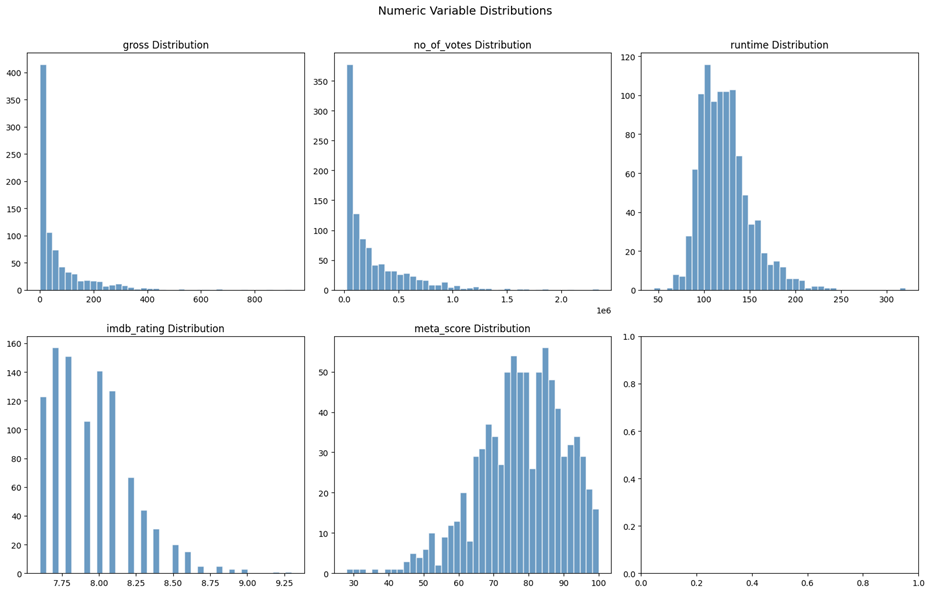
\includegraphics[width=0.7\linewidth]{figures/fig-1.png}
\end{figure}


\begin{figure}[!htbp]
    \centering
    \caption{Box plot distribution in numeric variables}
    \label{fig:2}
    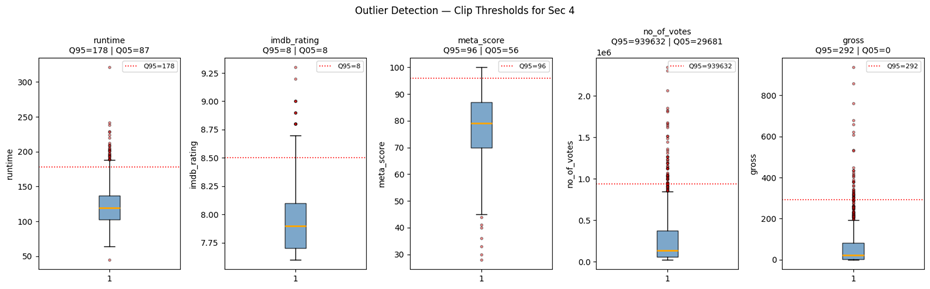
\includegraphics[width=0.7\linewidth]{figures/fig-2.png}
\end{figure}

\begin{figure}[!htbp]
        \centering
         \caption{Categorical coverage}
        \label{fig:3}
        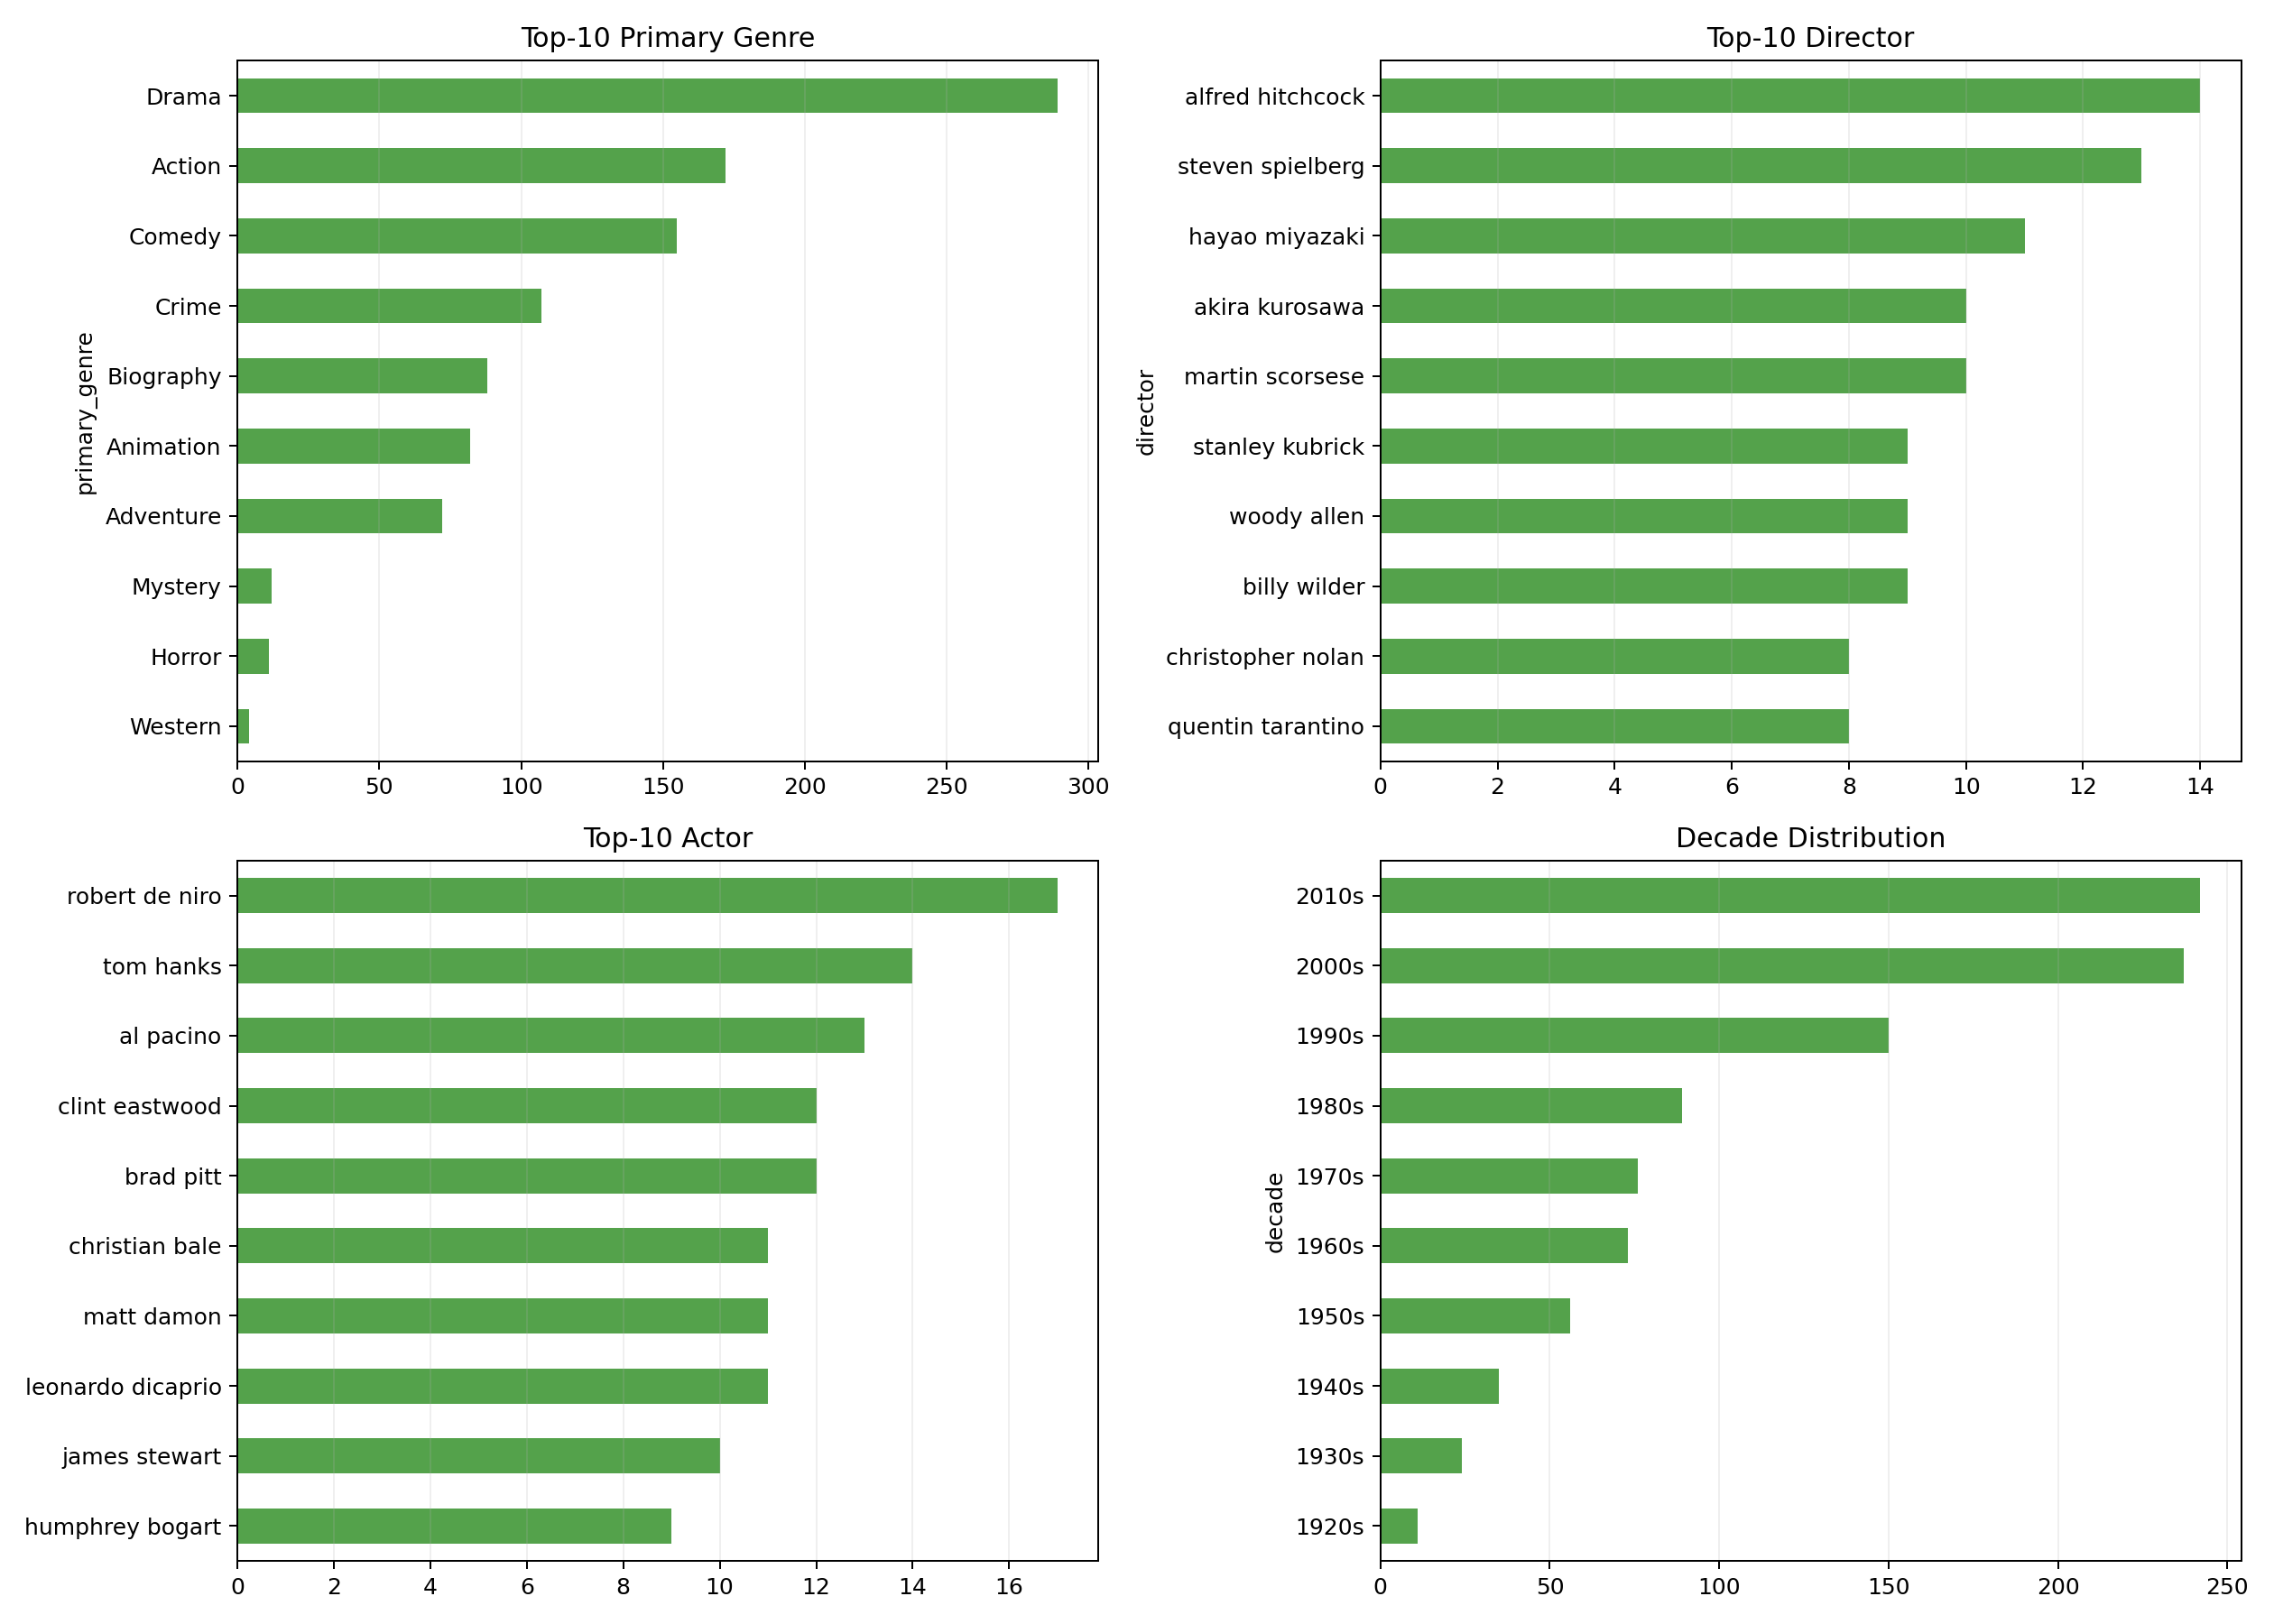
\includegraphics[width=0.7\linewidth]{figures/fig-3.png}
    \end{figure}       


The main data problems visible at this stage are: 
\begin{itemize}
    \item Inconsistent formatting for year, runtime, and gross
    \item Non-trivial missingness for revenue and external critic scores
    \item Composite genre strings that are not directly usable as categorical features.
\end{itemize}

\FloatBarrier

\subsubsection{Data Clean}

To make numeric fields analysis-ready, I apply the following transformations:

\begin{itemize}
    \item \verb|released_year|: parse to numeric, coercing errors to NaN; derive \texttt{decade} as \(\lfloor \text{year} / 10 \rfloor \times 10\), then label values as strings such as ``1990s''. Non-numeric years (1 row) are retained as NaN and excluded only from temporal summaries.
    \item \verb|runtime|: extract the numeric part from strings like ``142 min'' and cast to float minutes.
    \item \verb|gross|: remove thousands separators, cast to float, and divide by \(10^6\) to obtain millions of USD.
\end{itemize}

Rows with missing gross are not dropped; instead, I treat the missingness itself as informative (older and non-US productions) and exclude these rows only from revenue-based analyses. IMDB rating, Meta\_score, and number of votes are all coerced to numeric dtypes so they can be used in quantile-based tiering later. (Table 3 \ref{tab:3})
\begin{table}[!htbp]
    \caption{Skewness and Kurtosis of Key Numeric Variables}
    \centering
    \begin{tabular}{lrrrrr}
        \toprule
        \textbf{Variable} & \textbf{Mean} & \textbf{Median} & \textbf{Skewness} & \textbf{Kurtosis} & \textbf{Missing (\%)}\\
        \midrule
        runtime      & 122.89   & 119.00   & 1.21  & 3.43  & 0.0  \\
        imdb\_rating & 7.95     & 7.90     & 1.02  & 1.43  & 0.0  \\
        meta\_score & 77.97    & 79.00    & -0.61 & 0.42  & 15.7 \\
        no\_of\_votes & 273692.91 & 138548.50 & 2.30 & 6.90 & 0.0  \\
        gross        & 68.04    & 23.53    & 3.13  & 13.91 & 16.9 \\
        \bottomrule
    \end{tabular}
    \label{tab:3}
\end{table}

For categorical variables, I standardize all column names to lowercase snake\_case and clean simple categorical fields. The genre column, which contains comma-separated lists (e.g., Action, Crime, Drama), is split into:

\begin{itemize}
    \item \verb|genre_list|: a list of cleaned genre labels for each movie,
    \item \verb|primary_genre|: the first genre in the list, used in most of the EDA and rule interpretation.
\end{itemize}

After cleaning, the dataset retains all 1,000 films with (as noted in Table \ref{tab:4}):
\begin{itemize}
    \item \textbf{Actors}: 2,709 distinct actors, no duplicate rows, normalized to lowercase with trimmed whitespace
    \item \textbf{Average basket size}: 3.996 actors per movie
    \item \textbf{Missing data}: 16.9\% for Gross revenue, 15.7\% for Meta scores, 10.1\% for certificates
\end{itemize}

\begin{table}[!htbp]
    \caption{Categorical Variable Summary}
    \centering
    \begin{tabular}{lrrlrr}
        \toprule
        \textbf{Variable} & \textbf{Observed rows} & \textbf{Unique values} & \textbf{Top category} & \textbf{Top count} & \textbf{Top share (\%)} \\
        \midrule
        primary\_genre & 1000 & 14 & Drama  & 289 & 28.90 \\
        certificate    & 899  & 16 & U      & 234 & 26.03 \\
        decade         & 999  & 11 & 2010s  & 242 & 24.22 \\
        \bottomrule
    \end{tabular}
    \label{tab:4}
\end{table}


\FloatBarrier

\subsection{Association Rule Mining Approaches}

As mentioned, in this project, frequent pairs are the core computational bottleneck and the base for downstream rule generation. Candidate-pair growth directly drives runtime and memory use, especially at low support thresholds.  The next section will explain in detail how each algorithm is applied in my IMDB experiments.

Considering each basket is one movie and the items are either its four main actors (actor-only) or actors plus discretized feature tiers (enriched). In both settings the item universe is \(I\), with items such as \verb|actor:tom hanks| or \verb|gross_tier:high|, and each movie basket is \(T_i \subseteq I\).  

Let \(T = \{T_{1}, \ldots, T_{m}\}\) be a multiset of transactions over a universe of items \(I\).
A frequent itemset \(X \subseteq I\) satisfies:
\[
\operatorname{supp}(X)
= \frac{\left|\{\,i : X \subseteq T_{i}\,\}\right|}{m}
\;\ge\; \mathrm{minsup}.
\]

An association rule \(X \Rightarrow Y\) with \(X \cap Y = \emptyset\) is characterized by:

\[
\text{Support:}\quad
\operatorname{supp}(X \Rightarrow Y) = \operatorname{supp}(X \cup Y)
\]

\[
\text{Confidence:}\quad
\operatorname{conf}(X \Rightarrow Y)
= \frac{\operatorname{supp}(X \cup Y)}{\operatorname{supp}(X)}
\]

\[
\text{Lift:}\quad
\operatorname{lift}(X \Rightarrow Y)
= \frac{\operatorname{conf}(X \Rightarrow Y)}{\operatorname{supp}(Y)}
\]

\[
\text{Interest (leverage):}\quad
\operatorname{interest}(X \Rightarrow Y)
= \operatorname{supp}(X \cup Y)
- \operatorname{supp}(X)\,\operatorname{supp}(Y)
\]

In practice, the main bottleneck is counting candidate pairs, since their number can be very large even when only few larger itemsets are frequent. The objective is to find all subsets \(X \subseteq I\) that appear in at least a given number of movies (\verb|minsup|), and then derive association rules \(X \Rightarrow Y\) with high support, confidence, and lift. For example, in the actor-only setting a rule could be
\[
\{\texttt{actor:daniel radcliffe}\} \Rightarrow \{\texttt{actor:emma watson}\},
\]
indicating a strong co-casting pattern. In the enriched setting, a rule such as
\[
\{\texttt{actor:tom hanks}\} \Rightarrow \{\texttt{gross\_tier:high}\}
\]
captures an actor--success association. 

Because the number of possible itemsets is \(2^{|I|}\), I rely on three classical ARM algorithms to prune this search space efficiently on movie baskets.

Across all experiments the workflow is the same (see Figure \ref{fig:4}):
\begin{itemize}
    \item Build movie baskets from the cleaned IMDB table
    \item Mine frequent singletons and pairs (\(2\)-itemsets) with Apriori, PCY, or PCY-Multistage
    \item  Extend to larger itemsets (\(k \ge 3\)) using Apriori's join-and-prune step
    \item Generate association rules from the union of all frequent itemsets.
\end{itemize}

\begin{figure}[!htbp]
\centering
\caption{Main-memory flow of Apriori, PCY, and PCY-Multistage for pair mining on movie baskets.}
\label{fig:4}
\begin{subfigure}{0.25\linewidth}
    \centering
    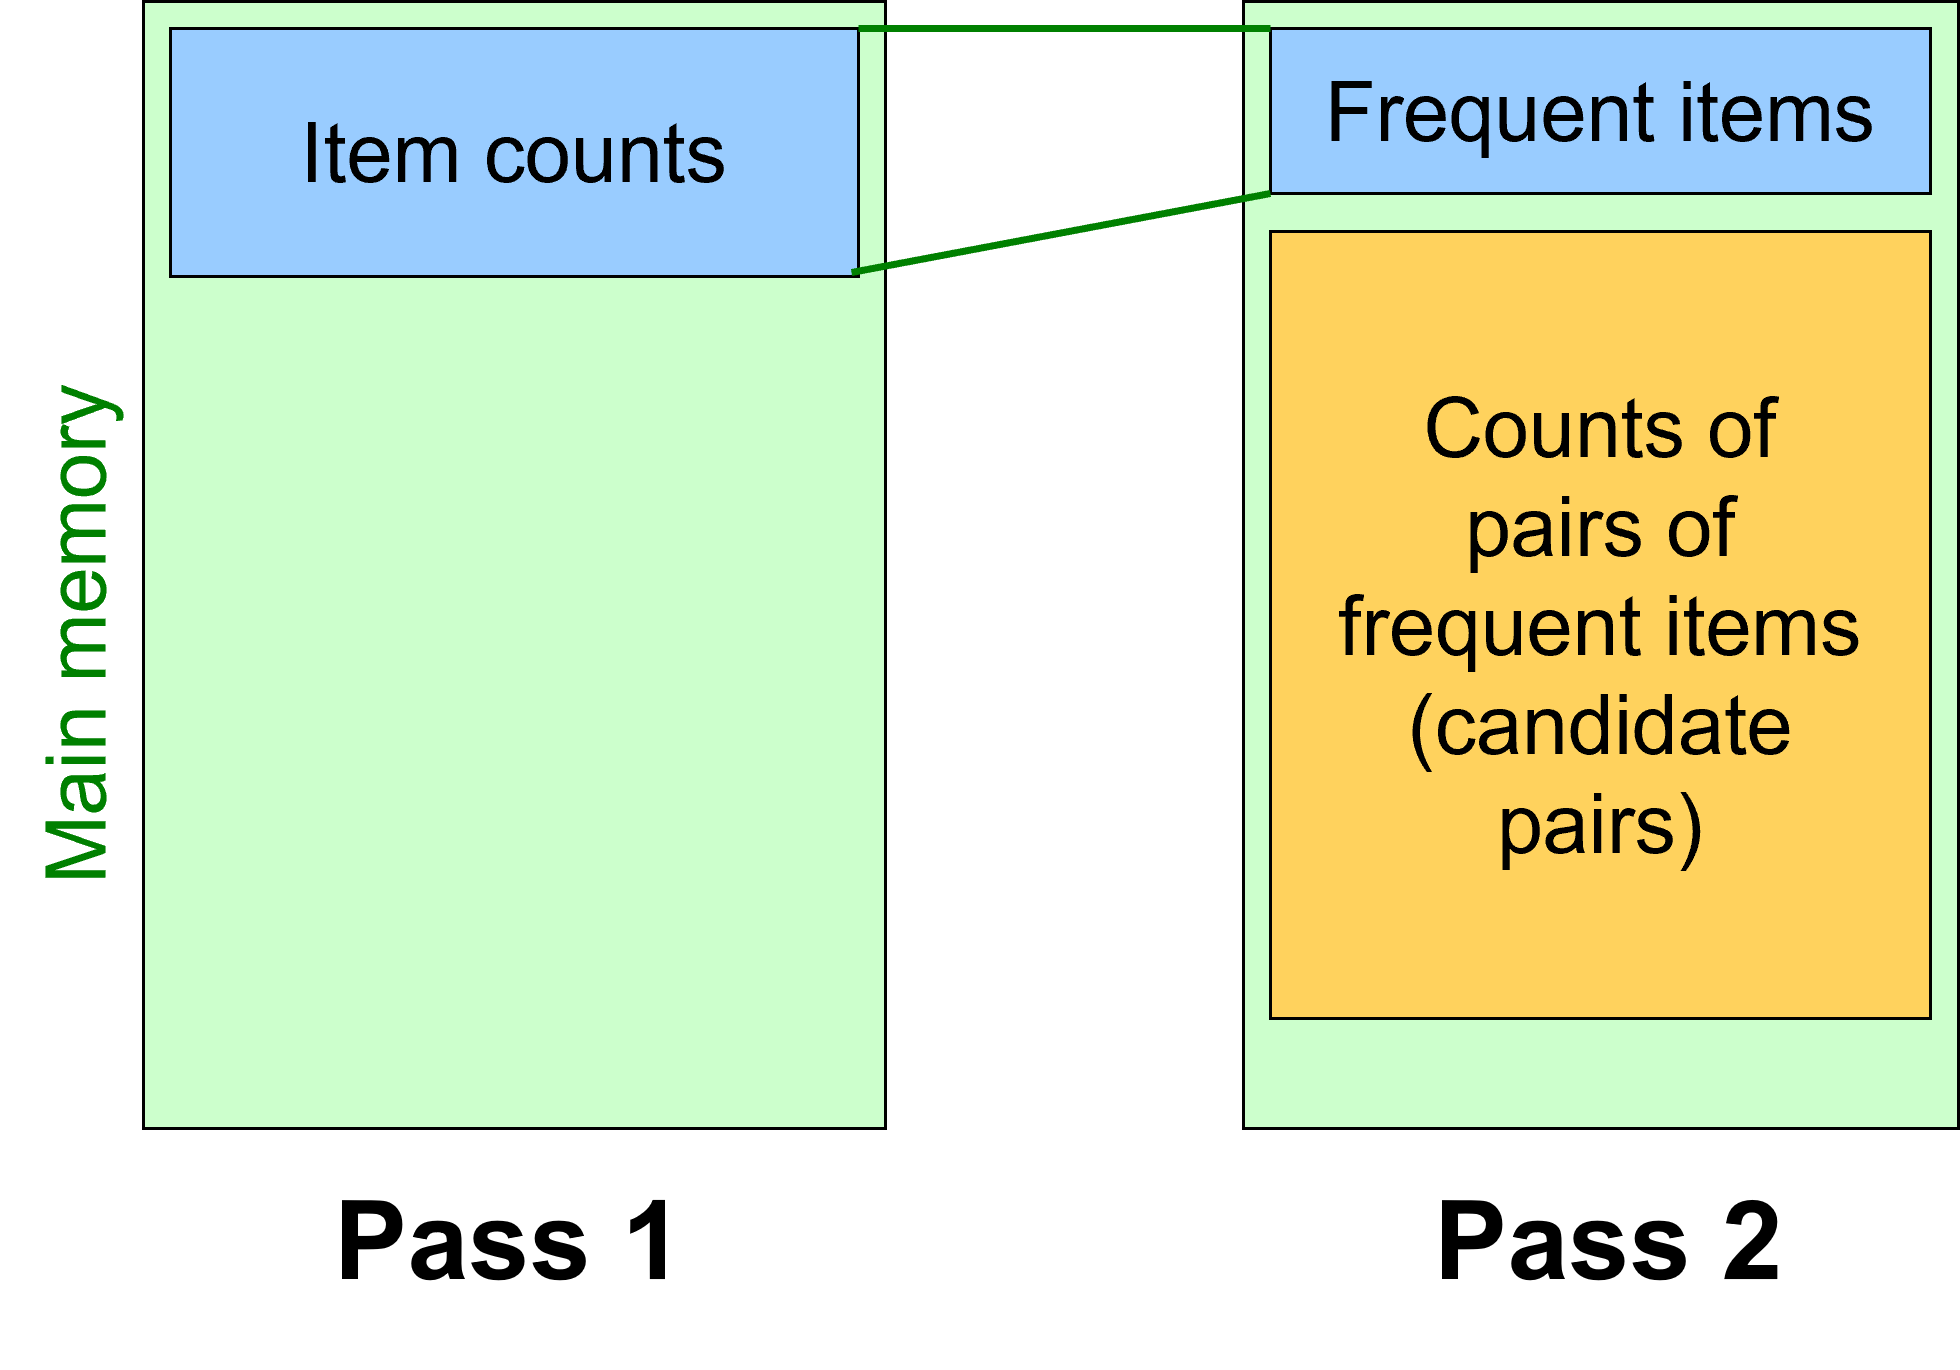
\includegraphics[width=\linewidth]{figures/apriori_main_memory.png}
    \caption{Apriori}
\end{subfigure}\hfill
\begin{subfigure}{0.25\linewidth}
    \centering
    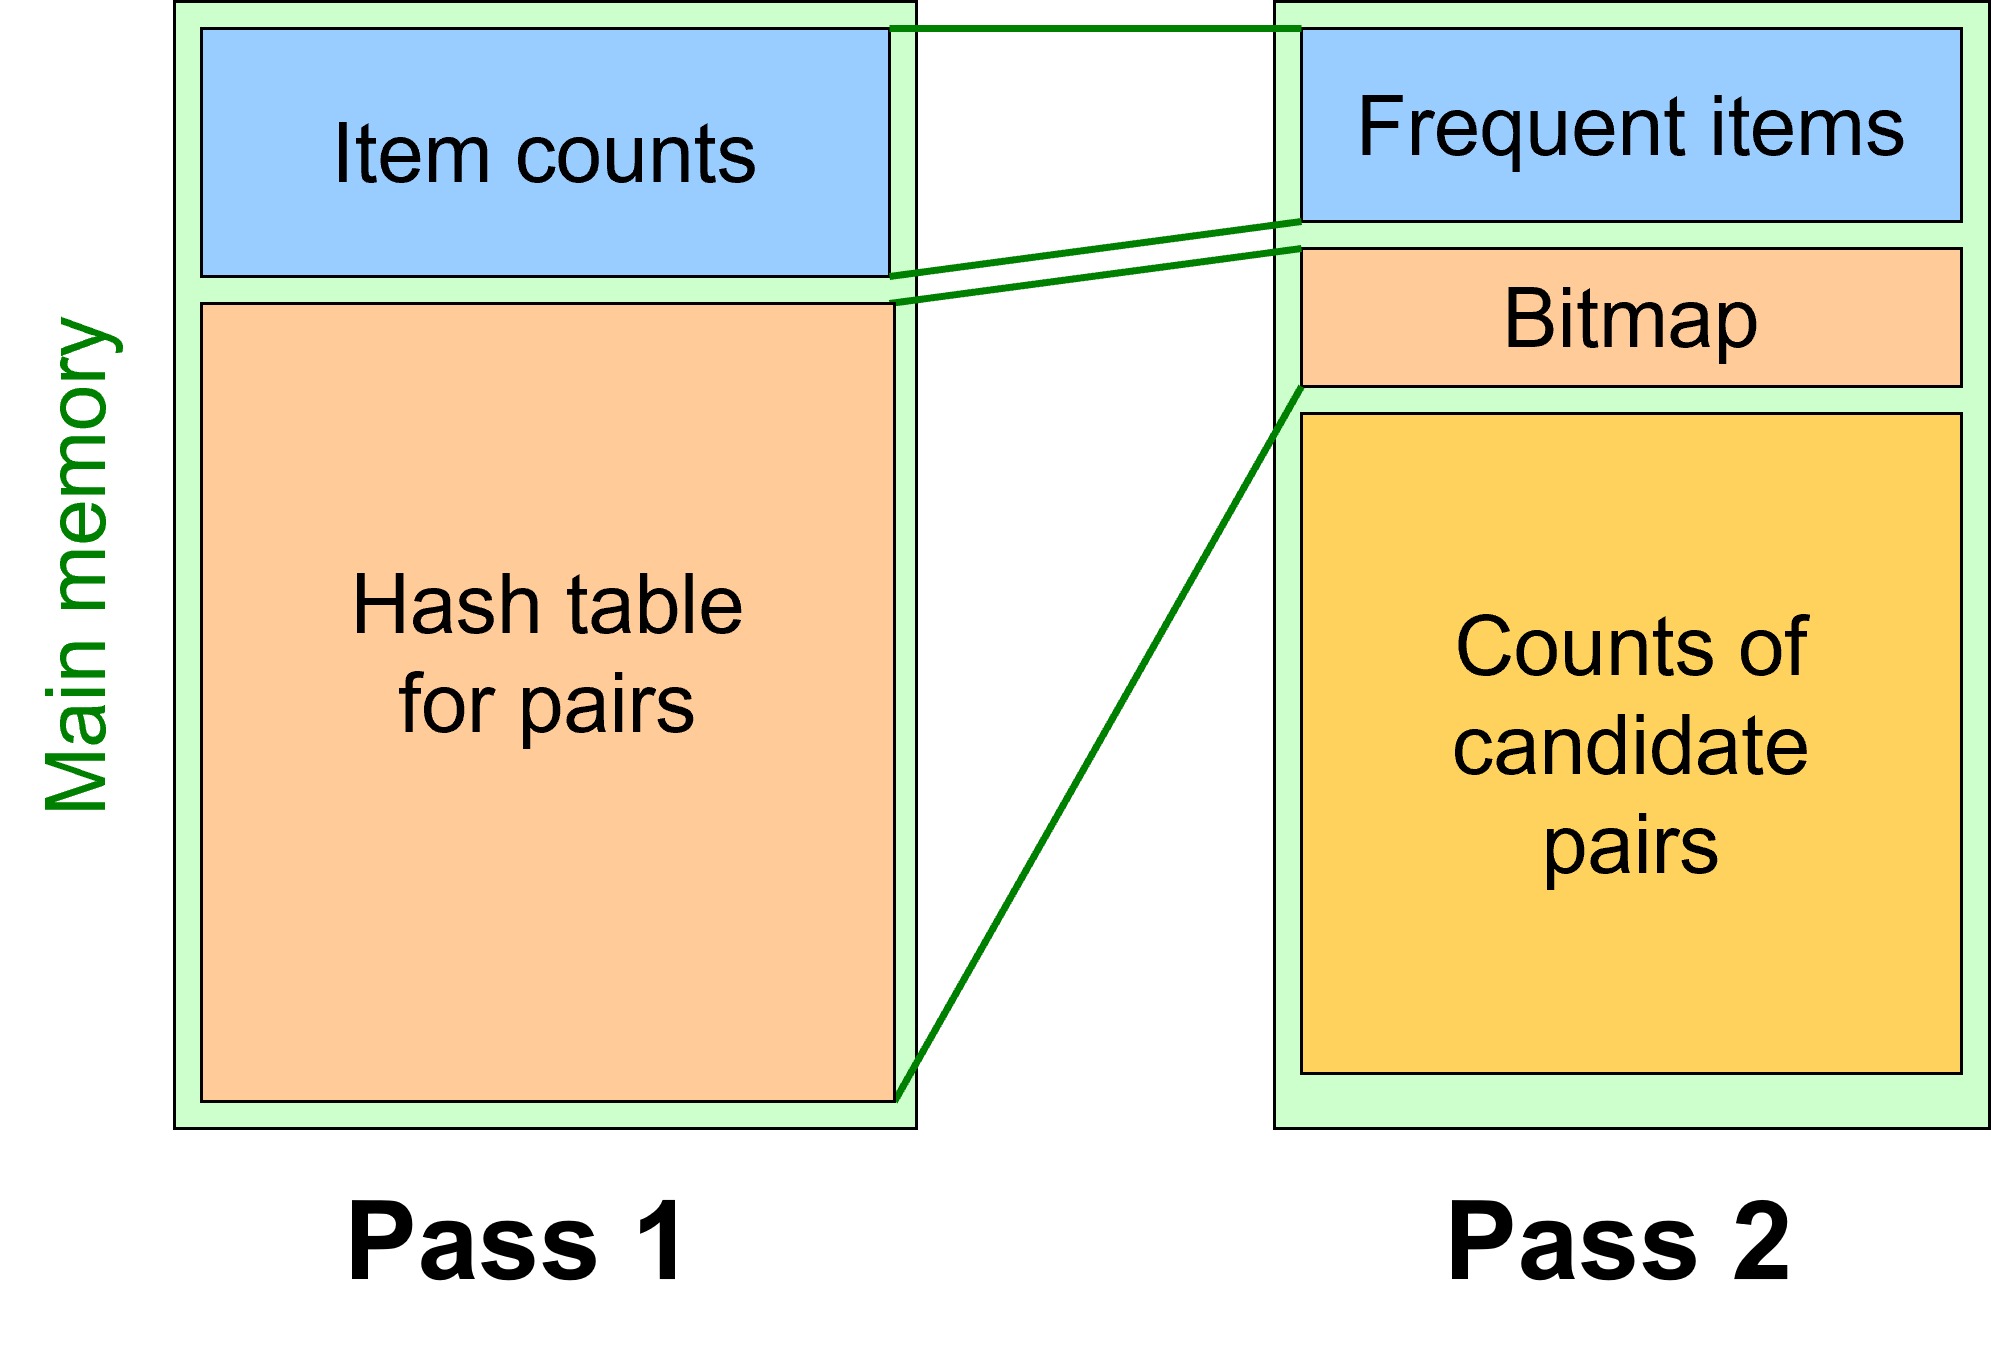
\includegraphics[width=\linewidth]{figures/pcy_main_memory.png}
    \caption{PCY}
\end{subfigure}\hfill
\begin{subfigure}{0.35\linewidth}
    \centering
    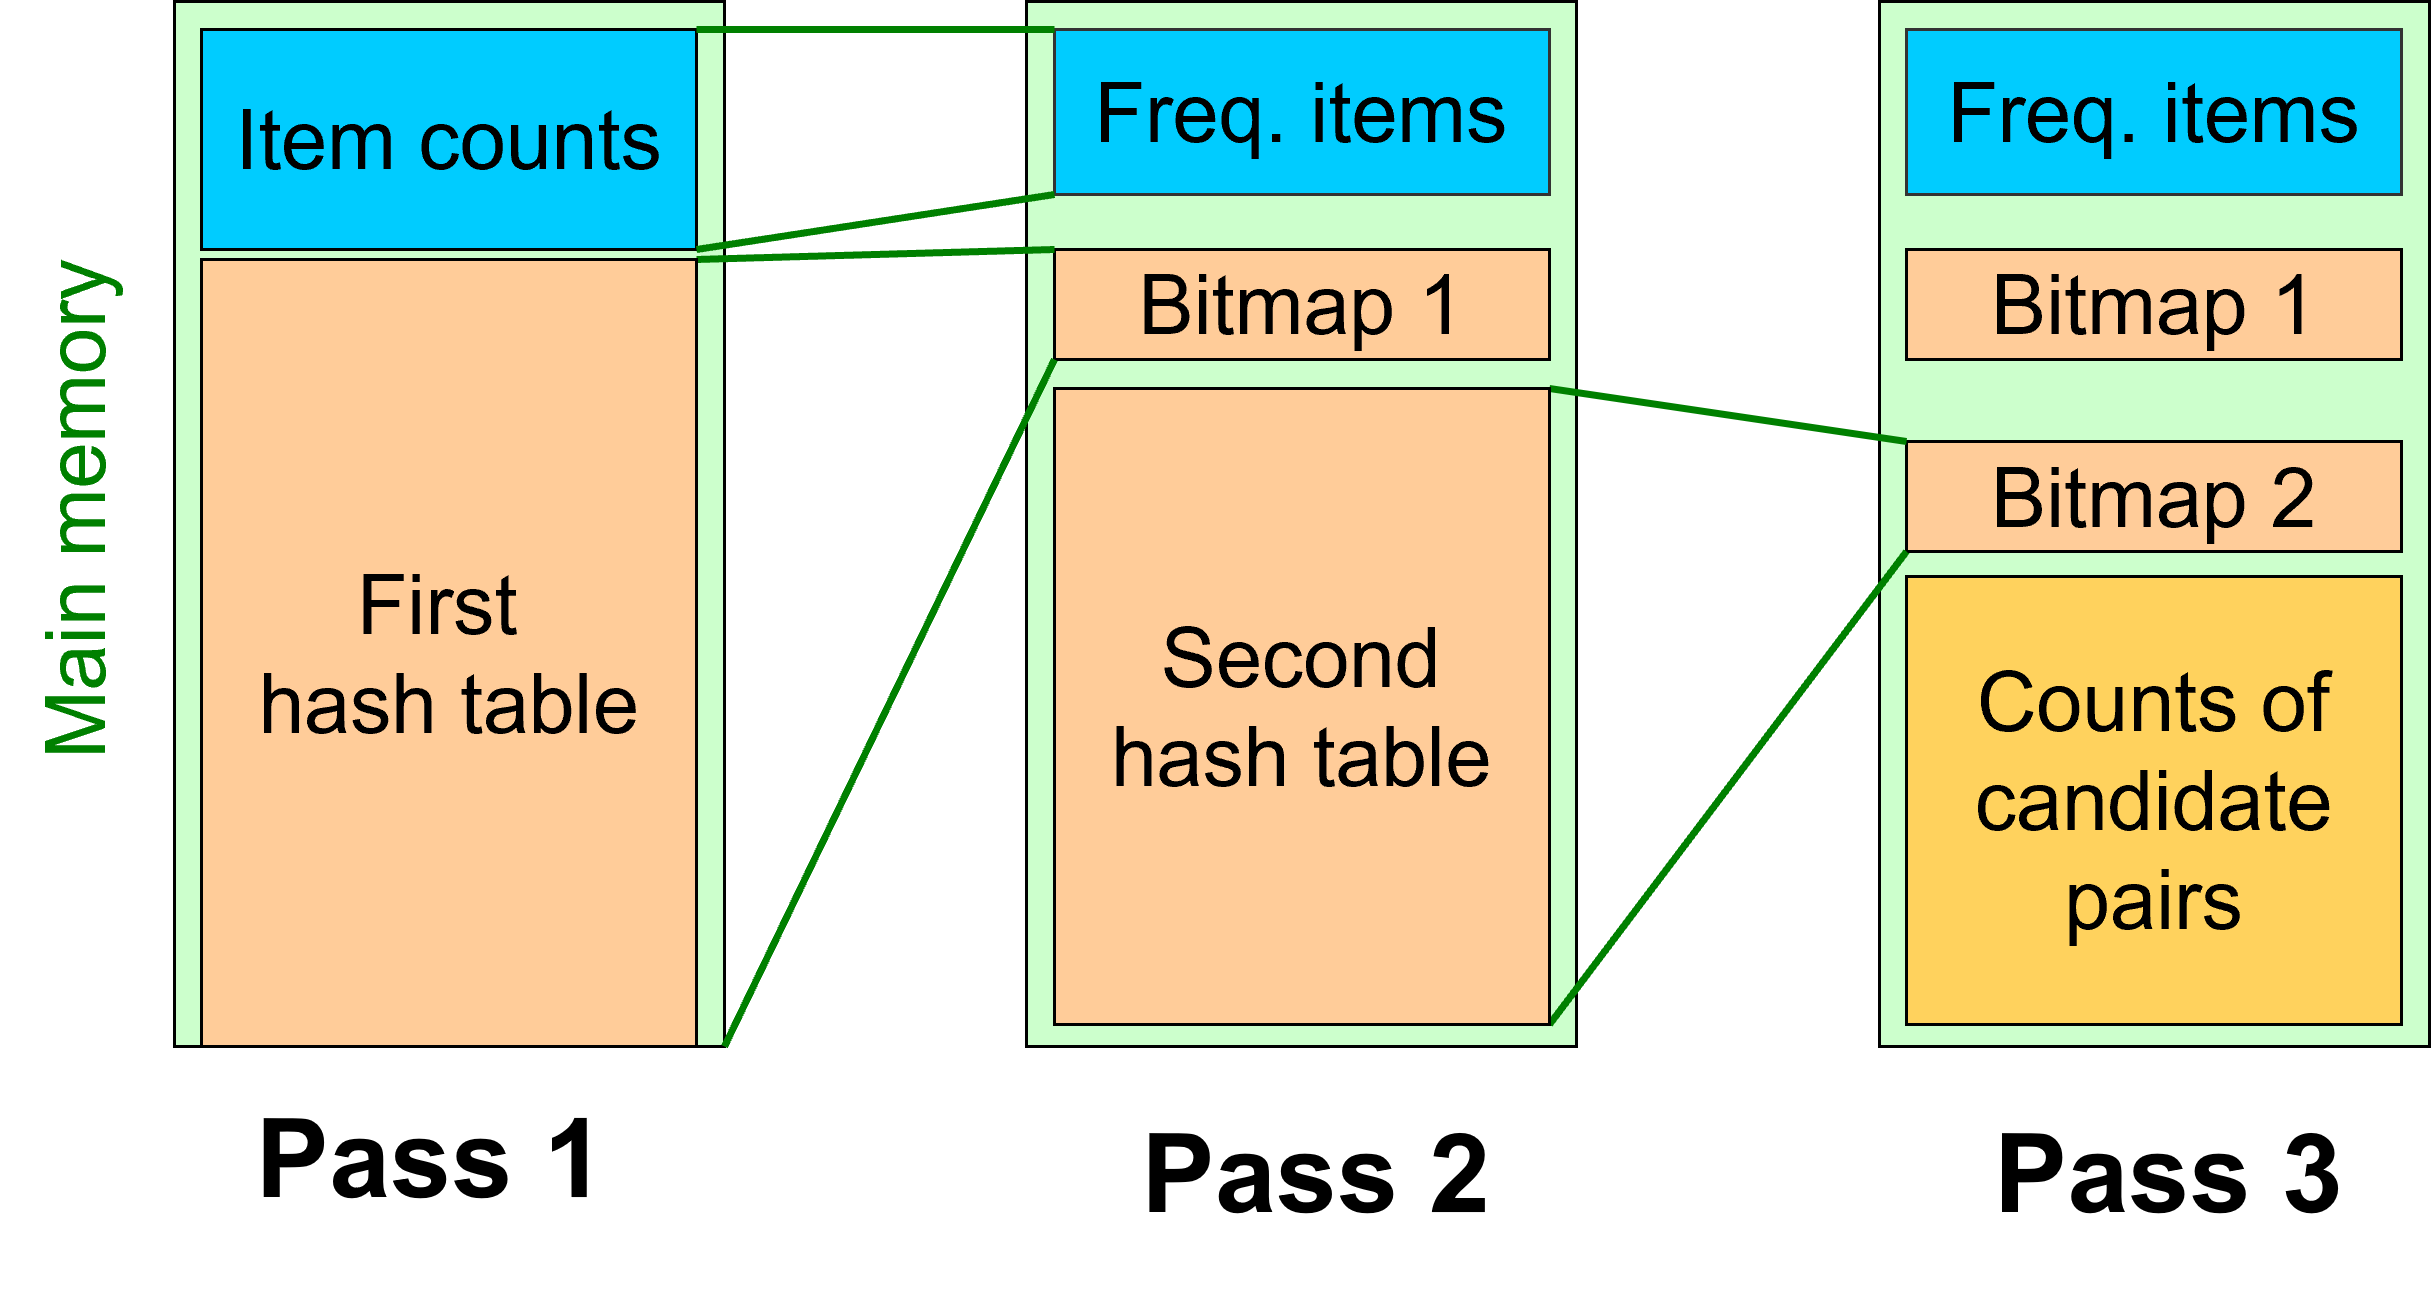
\includegraphics[width=\linewidth]{figures/pms_main_memory.png}
    \caption{PCY-Multistage (PMS)}
\end{subfigure}
\end{figure}

The pair-mining phase is the main computational bottleneck, so Section 4 compares algorithms primarily in terms of the number of candidate pairs they actually count (\(C_2\)) and the corresponding runtimes, on both actor-only and enriched movie baskets.

\subsubsection{Apriori on Movie Baskets}

Apriori is the classical level-wise frequent-itemset algorithm based on the downward-closure property: if an itemset \(X\) is frequent, then every subset of \(X\) must also be frequent. In the movie context this means, for example, that if the triple \textit{\{\texttt{actor:daniel radcliffe}, \texttt{actor:emma watson}, \texttt{actor:rupert grint}\}} is frequent, then each pair from this triple must also be frequent.

I implement the standard two-pass version for pairs over the actor-only and enriched baskets:
\begin{itemize}
\item \textbf{Pass 1 (frequent items):} scan all movie baskets once and count each item (actor or actor/feature token), then keep items with support \(\ge\) \verb|minsup| as \(L_1\).
\item \textbf{Pass 2 (frequent pairs):} for each basket, restrict to \(L_1\), generate unordered pairs \(\{i,j\}\), and count their supports; keep pairs with support \(\ge\) \verb|minsup| as \(L_2\).
\end{itemize}

For itemsets of size \(k \ge 3\), I use the textbook Apriori join-and-prune strategy (MMDS Algorithm 6.1): candidates \(C_k\) are built by joining frequent \((k-1)\)-itemsets in \(L_{k-1}\), removing candidates whose \((k-1)\)-subsets are not all in \(L_{k-1}\), then counting supports over all movie baskets to obtain \(L_k\). The detailed Apriori algorithm is shown below.

\paragraph{Apriori pseudocode (\texttt{run\_apriori\_full})}\mbox{}\\
\textbf{Input:} transaction database \(D\), minimum support \(\epsilon\), maximum size \(K\).\\
\textbf{Output:} frequent itemsets \(L[k]\) and support counts \(\mathrm{Cnt}[k]\).\\
\textbf{Method:}
    \begin{small}
    \begin{tabular}{@{}r p{0.90\linewidth}@{}}
    01 & Count all items in \(D\) to get singleton supports. \\
    02 & Build \(L_1 = \{\{i\}\mid \mathrm{support}(i)\ge \epsilon\}\); set \(L[1]\leftarrow L_1\), \(\mathrm{Cnt}[1]\leftarrow\) singleton counts. \\
    03 & If \(K>1\), generate all 2-item combinations from items in \(L_1\) as \(C_2\). \\
    04 & Count supports of \(C_2\) over all transactions and keep \(L_2=\{c\in C_2\mid \mathrm{support}(c)\ge \epsilon\}\). \\
    05 & Store \(L[2]\leftarrow L_2\), \(\mathrm{Cnt}[2]\leftarrow\) pair counts. \\
    06 & For \(k=3\) to \(K\): if \(L[k-1]\) is empty, stop. \\
    07 & Generate \(C_k\) by Apriori join-and-prune from \(L[k-1]\). \\
    08 & If \(C_k\) is empty, stop. \\
    09 & Count supports of all candidates in \(C_k\), then keep \(L_k=\{c\in C_k\mid \mathrm{support}(c)\ge \epsilon\}\). \\
    10 & Store \(L[k]\leftarrow L_k\), \(\mathrm{Cnt}[k]\leftarrow\) counts of \(C_k\). \\
    11 & Return all \(L[k]\) and \(\mathrm{Cnt}[k]\). \\
    \end{tabular}
\end{small}

For each configuration (basket design, \verb|minsup|, max \(k\)) I record:
\begin{itemize}
    \item \(|L_1|\): number of frequent single items,
    \item \(C_2^{\text{Apr}}\): number of distinct pairs whose support is counted in Pass 2,
    \item \(|L_2^{\text{Apr}}|\): number of frequent pairs found,
    \item \verb|time_Apr|: runtime of pair mining (Passes 1--2).
\end{itemize}
Higher-order counts \(|L_k|\) for \(k=3,4\) are also reported, but the main comparison with PCY and PCY-Multistage focuses on \(C_2\) and runtime.

\subsubsection{PCY: Hashing Pairs in Pass 1}

PCY (Park--Chen--Yu) is a memory-efficient refinement of Apriori that uses a hash-bucket bitmap to filter impossible candidate pairs before they are counted. Given a hash function \(h_1\) from unordered pairs to \(\{0, \dots, B-1\}\), the implementation is:
\begin{itemize}
    \item Pass 1 (frequent items + bucket counts): as in Apriori, scan all movies to obtain \(L_1\); at the same time, hash every observed pair \(\{i,j\}\) into bucket \(h_1(i,j)\) and increment bucket counts. After the scan, create Bitmap 1 where bucket \(b\) is marked frequent if its count is \(\ge\) \verb|minsup|.
    \item Pass 2 (filtered pair counting): for each movie, restrict to \(L_1\), generate pairs, and count a pair \(\{i,j\}\) only if its bucket \(h_1(i,j)\) is marked frequent in Bitmap 1.
\end{itemize}

The key intuition for this movie data is that many actor combinations (especially in enriched baskets) are extremely rare. If a bucket total is below \verb|minsup|, then every specific pair hashing into that bucket must be infrequent, so all those pairs can be skipped safely.

\paragraph{PCY pseudocode (\texttt{pcy\_full})}\mbox{}\\
\begin{small}
\textbf{Input:} transaction database \(D\), minimum support \(\epsilon\), maximum size \(K\), bucket count \(B\).\\
\textbf{Output:} frequent itemsets \(L[k]\), support counts \(\mathrm{Cnt}[k]\), and stage-1 bitmap.\\
\textbf{Method:}
\begin{tabular}{@{}r p{0.90\linewidth}@{}}
01 & Initialize singleton counter and stage-1 bucket counters of size \(B\). \\
02 & Pass 1 over \(D\): update singleton counts and hash each observed pair \((i,j)\) to bucket \(h_1(i,j)\). \\
03 & Build \(L_1=\{i\mid \mathrm{support}(i)\ge \epsilon\}\) and bitmap\(_1[b]=1\) if bucket count \(b\ge \epsilon\), else \(0\). \\
04 & Pass 2 over \(D\): for each transaction, keep only items in \(L_1\), generate pairs, and count a pair only if bitmap\(_1[h_1(i,j)] = 1\). \\
05 & Build \(L_2=\{p\mid \mathrm{support}(p)\ge \epsilon\}\). \\
06 & Convert \(L_1\) and \(L_2\) to set-form itemsets; store in \(L[1]\), \(L[2]\), with counts in \(\mathrm{Cnt}[1]\), \(\mathrm{Cnt}[2]\). \\
07 & For \(k=3\) to \(K\): if \(L[k-1]\) is empty, stop. \\
08 & Generate \(C_k\) from \(L[k-1]\) using Apriori join-and-prune; if empty, stop. \\
09 & Count supports of \(C_k\) over \(D\), keep frequent \(L_k\), and store in \(L[k]\), \(\mathrm{Cnt}[k]\). \\
10 & Return \(L[k]\), \(\mathrm{Cnt}[k]\), and bitmap\(_1\). \\
\end{tabular}
\end{small}

For each experiment I collect:
\begin{itemize}
    \item \(C_2^{\text{PCY}}\): number of distinct pairs that pass Bitmap 1 and are counted in Pass 2,
    \item \(|L_2^{\text{PCY}}|\): number of frequent pairs returned (empirically matching Apriori),
    \item \verb|time_PCY|: runtime of pair mining.
\end{itemize}

\subsubsection{PCY-Multistage: Two Hash Filters}

PCY-Multistage (PMS) extends PCY by applying two independent hash filters before final pair counting. This adds a second screening step for pairs that survive the first bitmap due to collisions.

Let \(h_1\) and \(h_2\) be two hash functions from unordered pairs to \(\{0, \dots, B-1\}\) \mbox{}\\
\begin{itemize}
    \item Pass 1 (Bitmap 1): compute \(L_1\), hash observed pairs with \(h_1\), and build Bitmap 1.
    \item Pass 2 (Bitmap 2): consider only pairs with items in \(L_1\) and frequent bucket in Bitmap 1; re-hash them with \(h_2\), then build Bitmap 2.
    \item Pass 3 (final pair counting): count a pair \(\{i,j\}\) only if both items are in \(L_1\), \(h_1(i,j)\) maps to a frequent bucket in Bitmap 1, and \(h_2(i,j)\) maps to a frequent bucket in Bitmap 2.
\end{itemize}

This reduces false-positive pair candidates from hash collisions. A pair must survive two independent bitmap checks before exact counting, which typically shrinks the counted candidate set more than single-stage PCY.


\begin{small}
\paragraph{PCY-Multistage pseudocode (\texttt{pcy\_multistage\_full})}\mbox{}\\
\noindent\textbf{Input:} transaction database \(D\), minimum support \(\epsilon\), maximum size \(K\), stage-1 buckets \(B_1\), stage-2 buckets \(B_2\).\\
\textbf{Output:} frequent itemsets \(L[k]\), support counts \(\mathrm{Cnt}[k]\), Bitmap 1, Bitmap 2.\\
\textbf{Method:}
\begin{tabular}{@{}r p{0.90\linewidth}@{}}
01 & Define two stage-specific hash functions \(h_1(i,j)\) and \(h_2(i,j)\). \\
02 & Pass 1: count singletons and stage-1 bucket totals; build \(L_1\) and Bitmap 1 (bucket frequent if count \(\ge \epsilon\)). \\
03 & Pass 2: for each transaction, keep unique items in \(L_1\); for each pair, keep it only if Bitmap 1 accepts it, then hash with \(h_2\) and update stage-2 buckets. \\
04 & Build Bitmap 2 from stage-2 bucket counts using the same threshold \(\epsilon\). \\
05 & Pass 3: scan transactions again; count a pair only if it passes all three checks: both items in \(L_1\), Bitmap 1 acceptance, and Bitmap 2 acceptance. \\
06 & Build \(L_2=\{p\mid \mathrm{support}(p)\ge \epsilon\}\), then store \(L[1]\), \(L[2]\), \(\mathrm{Cnt}[1]\), \(\mathrm{Cnt}[2]\). \\
07 & For \(k=3\) to \(K\): if \(L[k-1]\) is empty, stop. \\
08 & Generate \(C_k\) with Apriori join-and-prune; if empty, stop. \\
09 & Count supports of \(C_k\), keep frequent \(L_k\), and store in \(L[k]\), \(\mathrm{Cnt}[k]\). \\
10 & Return \(L[k]\), \(\mathrm{Cnt}[k]\), Bitmap 1, and Bitmap 2. \\
\end{tabular}
\end{small}

For each configuration I track:
\begin{itemize}
    \item \(C_2^{\text{PMS}}\): number of distinct pairs that survive both bitmaps and are counted in Pass 3,
    \item \(|L_2^{\text{PMS}}|\): number of frequent pairs found (empirically matching Apriori and PCY),
    \item \verb|time_PMS|: runtime of the three-pass pair-mining stage.

\end{itemize}
Section 4 compares \(C_2\) and runtime side by side for Apriori, PCY, and PMS on both actor-only baskets (four actors per movie) and enriched baskets (actors plus tier items), to quantify the practical gain from one-stage and two-stage hashing over the Apriori baseline.
 
\FloatBarrier

\subsection{Features Engineering}

\subsubsection{Actors Variable}

The main modeling decision for frequent-itemset mining is to treat each movie as a basket and its main actors as items. I construct actor-only baskets as follows:
\begin{itemize}
    \item Normalize actor names in star1 : star4: strip whitespace, lowercase, and prefix with \verb|actor:| (e.g., ``Tom Hanks'' \(\rightarrow\) \verb|actor:tom hanks|).
    \item For each movie, collect these four names, drop NaNs (none in this dataset), and remove duplicates within the movie, then store them as an unordered set.
    \item Discard movies that would end up with an empty basket (none here).
\end{itemize}

This yields an actor-only basket dataset with:
\begin{itemize}
    \item 1000 baskets (movies),
    \item exactly 4 items per basket in almost all cases,
    \item several thousand distinct actor items in the global universe.
\end{itemize}
(See Table \ref{tab:5} and Table \ref{tab:6}.)

\begin{table}[!htbp]
    \caption{Top 10 Actors by Appearance Frequency}
    \centering
    \begin{tabular}{llr}
        \toprule
        \textbf{Rank} & \textbf{Actor} & \textbf{Count} \\
        \midrule
        1  & Robert De Niro      & 17 \\
        2  & Tom Hanks           & 14 \\
        3  & Al Pacino           & 13 \\
        4  & Brad Pitt           & 12 \\
        5  & Clint Eastwood      & 12 \\
        6  & Christian Bale      & 11 \\
        7  & Leonardo DiCaprio   & 11 \\
        8  & Matt Damon          & 11 \\
        9  & James Stewart       & 10 \\
        10 & Humphrey Bogart     & 9 \\       
        \bottomrule
    \end{tabular}
    \label{tab:5}
\end{table}
\begin{table}[!htbp]
    \caption{Basket-Level Summary for Actor--Movie Data}
    \centering
    \begin{tabular}{p{0.60\textwidth}r}
        \toprule
        \textbf{Metric} & \textbf{Value} \\
        \midrule
        n\_baskets & 1000 \\
        n\_distinct\_actors & 2709 \\
        basket\_size\_min & 3 \\
        basket\_size\_mean & 4.00 \\
        basket\_size\_max & 4 \\
        max\_actor\_frequency & 17 \\
        actors\_with\_ge\_8\_movies & 17 \\
        \bottomrule
    \end{tabular}
    \label{tab:6}
\end{table}


\FloatBarrier

\subsubsection{Enriched variables}

To study how the algorithms behave when the itemspace is larger and baskets contain heterogeneous features, I also construct an enriched basket representation. For each movie I retain the four actor items and add one discretized tier item for each of several numeric variables:

\begin{itemize}
    \item gross\_tier (e.g., low/mid/high by quantiles),
    \item rating\_tier (buckets of IMDB rating),
    \item meta\_score\_tier,
    \item votes\_tier,
    \item runtime\_tier.
\end{itemize}

Each tier is encoded as an item like \verb|gross_tier:high| or \verb|votes_tier:low|, so a typical enriched basket contains 4 actor items plus 4--5 tier items. The enriched basket space therefore has:

\begin{itemize}
    \item the same 1000 movies,
    \item a significantly larger item universe (actors + feature tiers),
    \item larger average basket size and a much denser candidate pair space.
\end{itemize}

\begin{table}[!htbp]
    \caption{Enriched Basket and Tier Item Summary}
    \centering
    \begin{tabular}{ll}
        \toprule
        \textbf{Metric} & \textbf{Value} \\
        \midrule
        n\_baskets          & 1000 \\
        items\_universe     & 2724 \\
        basket\_size\_min   & 7 \\
        basket\_size\_mean  & 8.67 \\
        basket\_size\_max   & 9 \\
        top\_tier\_item\_1  & rating\_tier:low (431) \\
        top\_tier\_item\_2  & runtime\_tier:low (343) \\
        top\_tier\_item\_3  & runtime\_tier:mid (339) \\
        top\_tier\_item\_4  & votes\_tier:low (334) \\
        top\_tier\_item\_5  & votes\_tier:high (333) \\
        top\_tier\_item\_6  & votes\_tier:mid (333) \\
        top\_tier\_item\_7  & rating\_tier:high (322) \\
        top\_tier\_item\_8  & runtime\_tier:high (318) \\
        top\_tier\_item\_9  & meta\_score\_tier:low (284) \\
        top\_tier\_item\_10 & meta\_score\_tier:mid (282) \\
        \bottomrule
    \end{tabular}
    \label{tab:7}
\end{table}


This enriched representation is used solely to stress-test candidate generation, as discussed in the next section, showing that the relative advantage of PCY and especially PCY-Multistage in terms of \(C_2\) reduction and runtime becomes much more visible when the item universe and basket size increase, even though the underlying IMDB data remain the same.
 


\FloatBarrier

\section{Experimental Setup and Results}

This section describes how I configure and run Apriori, PCY, and PCY-Multistage on IMDB movie baskets, and how candidate counts and runtimes are used to compare configurations for each basket design. All experiments are executed in a single Python notebook (\texttt{experiment-code-v4.0}) with shared preprocessing and fixed reproducibility settings.

\subsection{Reproducibility and Common Settings}

All experiments share the same environment settings:
\begin{itemize}
    \item Dataset and preprocessing: cleaned IMDB Top-1000 table from Sections 1--4, with normalized actor names and engineered tier features.
    \item Random seed: \verb|SEED = 42| for Python \verb|random| and NumPy.
    \item Bucket configuration: \verb|DEFAULT_NUM_BUCKETS = 2048| for PCY and PCY-Multistage (both hash stages in PMS use 2048 buckets).
    \item Timing protocol: wall-clock time measured with \verb|time.perf_counter| around pair-mining passes only, so one-off data loading/cleaning does not affect algorithm comparison.
\end{itemize}

\subsection{Basket Designs and Minsup Grids}

\subsubsection*{Actor-only baskets}
For the actor-only design, each movie is represented as a basket of up to four actors (\verb|star1|--\verb|star4|) after cleaning and normalization as reported in Table~\ref{tab:6}. I use a relative support grid \(\{0.002,\allowbreak 0.003,\allowbreak 0.005,\allowbreak 0.007\}\), which maps to absolute \(\mathrm{minsup}\) values \(\{2,\allowbreak 3,\allowbreak 5,\allowbreak 7\}\) since \(m = 1000\), and cap Apriori-style expansion at \(k_{\max} = 4\) to match the maximum basket width.

\subsubsection*{Enriched baskets}

For the enriched design, each movie basket contains the actor items plus five compact tier features (\verb|gross_tier|, \verb|votes_tier|, \verb|rating_tier|, \verb|runtime_tier|, \verb|meta_score_tier|), which increases basket width and the density of the pair space (see Table~\ref{tab:7}). Here I use a broader support grid aligned with the notebook outputs: absolute \(\mathrm{minsup}\)
 values \(\{2,\allowbreak 5,\allowbreak 10,\allowbreak 30,\allowbreak 50\}\), corresponding to ratios \(\{0.002,\allowbreak 0.005,\allowbreak 0.010,\allowbreak 0.030,\allowbreak 0.050\}\), and allow Apriori-style expansion up to \(k_{\max} = 9\), which is the maximum observed enriched basket size. 

\subsection*{Evaluation metrics and selection criterion}

\subsubsection{Metrics}
For each dataset, support threshold, and algorithm, I record:
\begin{itemize}
    \item \(C_{2}\): number of candidate pairs actually counted during the
    pair-mining phase.
    \item \(|L_{2}|\): number of frequent pairs returned at that
    \(\mathrm{minsup}\).
    \item \verb|time_pair|: pair-mining runtime (Apriori passes 1--2,
    PCY passes 1--2, PMS passes 1--3).
\end{itemize}
As a consistency check, I also track \(|L_{k}|\) and \(C_{k}\) for \(k \ge 3\) from the Apriori expansion, to verify that higher-order behavior matches the expected sparsity pattern. 

\subsubsection{Selection rule}

To compare configurations, I apply the following
decision rule:
\begin{enumerate}
    \item Retain only configurations that reproduce the same \(|L_{2}|\) as   Apriori at the same \(\mathrm{minsup}\) (correctness constraint).
    \item Among those, prefer the configuration with smaller \(C_{2}\)   (stronger candidate pruning).
    \item If \(C_{2}\) ties, choose the configuration with lower \verb|time_pair|.

\end{enumerate}

The definitions and formulas for the underlying rule-quality measures are
summarized in Table~\ref{tab:8}. 
\begin{table}[!htbp]
    \caption{Summary of Association Rule Evaluation Metrics}
    \centering
    \normalsize
    \begin{tabularx}{\textwidth}{lXX}
        \toprule
        \textbf{Metric} & \textbf{Definition} & \textbf{Formula / computation} \\
        \midrule
        Support &
        Fraction of baskets containing \(X\) &
        \(\displaystyle
        \mathrm{supp}(X)=\frac{\mathrm{supp\_count}(X)}{m}
        \) \\
        Confidence &
        Fraction of \(X\)-baskets that also contain \(Y\) &
        \(\displaystyle
        \mathrm{conf}(X \Rightarrow Y)=\frac{\mathrm{supp}(X \cup Y)}{\mathrm{supp}(X)}
        \) \\
        Interest (leverage) &
        Excess co-occurrence above what independence predicts &
        \(\displaystyle
        \mathrm{interest}(X \Rightarrow Y)=\mathrm{supp}(X \cup Y)-\mathrm{supp}(X)\,\mathrm{supp}(Y)
        \) \\
        Lift &
        How many times more often \(X\) and \(Y\) co-occur than under independence &
        \(\displaystyle
        \mathrm{lift}(X \Rightarrow Y)=\frac{\mathrm{conf}(X \Rightarrow Y)}{\mathrm{supp}(Y)}
        =\frac{\mathrm{supp}(X \cup Y)}{\mathrm{supp}(X)\,\mathrm{supp}(Y)}
        \) \\
        \bottomrule
    \end{tabularx}
    \label{tab:8}
\end{table}

\subsection{Experiment Results}

\subsubsection{Algorithm behavior on actor-only baskets}

On actor-only baskets, Apriori and PCY always produce identical frequent itemsets \(L_1\) and \(L_2\) at a given support threshold (Table \ref{tab:9actors_Lk_apr_pcy}), which confirms that hash-based pruning in PCY does not change correctness. The difference lies in how many candidates each method has to examine: while both algorithms consider all 2709 items as candidates in \(C_1\), PCY consistently reduces the number of candidate pairs \(C_2\) relative to Apriori (Table \ref{tab:10actors_Ck_apr_pcy}), with reductions growing from about 5\% at minsup = 2 to more than 90\% at minsup = 7.

PMS (Multistage PCY) pushes this idea further by using a second hash stage, and the effect is visible in Table \ref{tab:11pms_c2_drop}: at minsup = 5, it reduces \(C_2\) from 139 (Apriori) to only 3 candidate pairs, i.e., it is almost counting only truly frequent pairs. Table \ref{tab:12pcy_candidate_reduction} and Figure \ref{fig:5} summarize these candidate-level savings: PCY removes a modest but consistent fraction of the Apriori candidates, whereas PMS removes a large majority of them at low supports, especially when \(\mathrm{minsup\_ratio} \le 0.005\).

These reductions translate into large runtime effects. As shown in Table~\ref{tab:13runtime_speedup_enriched} and Figure~\ref{fig:6}, both PCY and PMS achieve orders-of-magnitude speedups over Apriori at low support for example, at \(\mathrm{minsup\_ratio} = 0.002\), PCY and PMS are more than
\(10^{2}\text{--}10^{3}\) times faster than Apriori—while speedups shrink to
single-digit factors when support is higher and the candidate space is small.
Conceptually, this behavior matches the design of the algorithms: when many
pairs are potential candidates, hash-based pruning (PCY, PMS) pays off; when
few remain, the overhead of hashing and extra passes dominates.

\begin{table}[!htbp]
    \caption{Apriori vs.\ PCY on Actor-Only Baskets: Frequent Itemsets \(L_k\)}
    \centering
    \begin{tabular}{rrrrrr}
        \toprule
        \textbf{minsup\_ratio} & \textbf{minsup} &
        \textbf{L1\_Apr} & \textbf{L2\_Apr} &
        \textbf{L1\_PCY} & \textbf{L2\_PCY} \\
        \midrule
        0.002 & 2 & 641 & 121 & 641 & 121 \\
        0.003 & 3 & 271 &  25 & 271 &  25 \\
        0.005 & 5 &  79 &   3 &  79 &   3 \\
        0.007 & 7 &  30 &   0 &  30 &   0 \\
        \bottomrule
    \end{tabular}
    \label{tab:9actors_Lk_apr_pcy}
\end{table}

\begin{table}[!htbp]
    \caption{Apriori vs.\ PCY on Actor-Only Baskets: Candidate Itemsets \(C_k\)}
    \centering
    \begin{tabular}{rrrrrrrr}
        \toprule
        \textbf{minsup\_ratio} & \textbf{minsup} &
        \textbf{C1\_Apr} & \textbf{C2\_Apr} &
        \textbf{C1\_PCY} & \textbf{C2\_PCY}  &\textbf{C2 drop} 
 &\textbf{C2 drop (\%)} 
\\
        \midrule
        0.002 & 2 & 2709 & 1516 & 2709 & 1439  &77 
 &5.08 
\\
        0.003 & 3 & 2709 &  622 & 2709 &  501  &121 
 &19.45 
\\
        0.005 & 5 & 2709 &  139 & 2709 &   51  &88 
 &63.31 
\\
        0.007 & 7 & 2709 &   32 & 2709 &    3  &29  &90.62 \\
        \bottomrule
    \end{tabular}
    \label{tab:10actors_Ck_apr_pcy}
\end{table}
\begin{table}[!htbp]
    \caption{PMS Candidate Reduction at the Pair Level (Actor-Only Baskets)}
    \centering
    \begin{tabular}{rrrrrrrr}
        \toprule
        \textbf{minsup\_ratio} & \textbf{minsup} &
         \textbf{C1\_Apr} 
&\textbf{C2\_Apr} &  \textbf{C1\_PMS}&\textbf{C2\_PMS} &
        \textbf{C2 drop} & \textbf{C2 drop (\%)} \\
        \midrule
        0.002 & 2 &  2709 
&1516 &  2709 
&795 & 721 & 47.56 \\
        0.003 & 3 &   2709 
&622 &   2709 
&69 & 553 & 88.91 \\
        0.005 & 5 &   2709 
&139 &    2709 
&3 & 136 & 97.84 \\
        0.007 & 7 &    2709 &32 &    2709 &0 &  32 & 100.00 \\
        \bottomrule
    \end{tabular}
    \label{tab:11pms_c2_drop}
\end{table}

\begin{table}[!htbp]
     \caption{PCY Candidate Reduction Relative to Apriori (Actor-Only Baskets)}
    \centering
    \begin{tabular}{rrrrrrrr}
        \toprule
        \textbf{minsup\_ratio} & \textbf{minsup} &
        \textbf{C2\_Apr} & \textbf{C2\_PMS}& \textbf{C2 drop} & \textbf{C2 drop (\%)} &
        \textbf{C3\_Apr} & \textbf{C3\_PCY} \\
        \midrule
        0.002 & 2 & 1516 & 1439 &  77 &  5.08 & 26 & 26 \\
        0.003 & 3 &  622 &  501 & 121 & 19.45 &  4 &  4 \\
        0.005 & 5 &  139 &   51 &  88 & 63.31 &  1 &  1 \\
        0.007 & 7 &   32 &    3 &  29 & 90.62 &  0 &  0 \\
        \bottomrule
    \end{tabular}
    \label{tab:12pcy_candidate_reduction}
\end{table}

\begin{figure}[!htbp]
    \centering
    \caption{Comparison of Candidate generation reduction (Actor-only Baskets). 
    (\subref{fig:5a}) PCY vs Apriori 
    (\subref{fig:5b}) PMS vs Apriori }
    \label{fig:5}
    \begin{subfigure}{0.5\textwidth}
        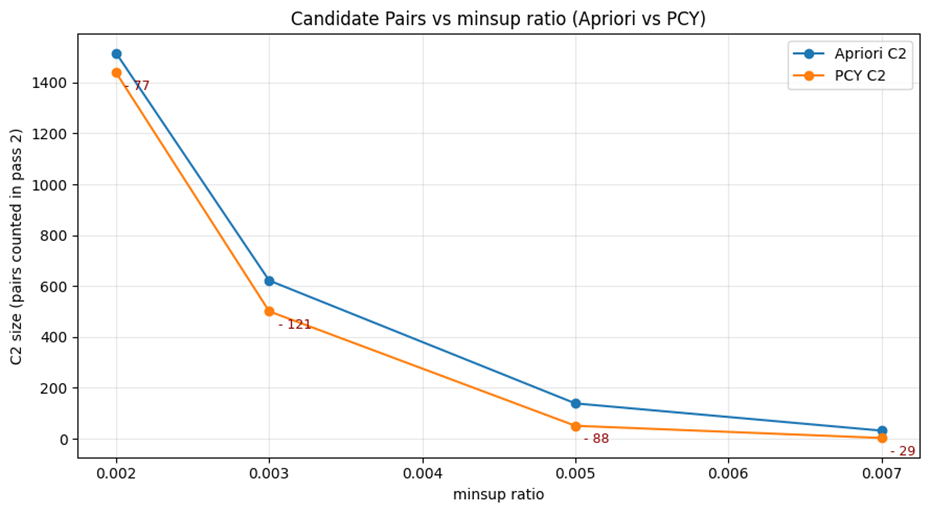
\includegraphics[width=\textwidth, height=2in]{figures/fig-5a.png}
        \caption{Candidate generation reduction of PCY relative to Apriori.}
        \label{fig:5a}
    \end{subfigure}
    \hfill
    \begin{subfigure}{0.5\textwidth}
           
         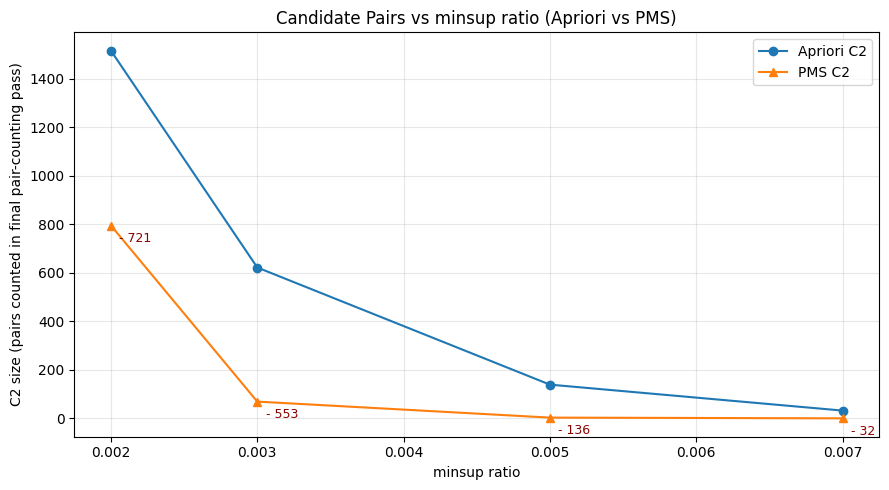
\includegraphics[width=\linewidth]{figures/fig-5b.png}
         \caption{Candidate generation reduction of PMS relative to Apriori}
         \label{fig:5b}
\end{subfigure}
\end{figure}
\begin{table}[!htbp]
    \caption{Runtime and Speedup of PCY and PMS Relative to Apriori (Actor-only Baskets)}
    \centering
    \normalsize
    \setlength{\tabcolsep}{3pt}
    \renewcommand{\arraystretch}{1.08}
    \begin{tabularx}{\textwidth}{>{\centering\arraybackslash}p{0.11\textwidth} >{\centering\arraybackslash}p{0.08\textwidth} >{\centering\arraybackslash}X >{\centering\arraybackslash}X >{\centering\arraybackslash}X >{\centering\arraybackslash}X >{\centering\arraybackslash}X}
        \toprule
        \textbf{minsup\_ratio} & \textbf{minsup} &
        \textbf{time\_Apriori (s)} &
        \textbf{time\_PCY (s)} &
        \textbf{time\_PMS (s)} &
        \textbf{speedup\_PCY / Apriori} &
        \textbf{speedup\_PMS / Apriori} \\
        \midrule
        0.002 & 2 & 90.69 & 0.0398 & 0.1950 & 2277.08 & 465.10 \\
        0.003 & 3 & 18.21 & 0.0403 & 0.0340 &  452.25 & 535.44 \\
        0.005 & 5 &  0.79 & 0.0237 & 0.0289 &   33.34 &  27.31 \\
        0.007 & 7 &  0.13 & 0.0206 & 0.0336 &    6.43 &   3.94 \\
        \bottomrule
    \end{tabularx}
    \label{tab:13runtime_speedup_enriched}
\end{table}


\begin{figure}
 \caption{Runtime performance at different support threshold (Apriori vs PCY vs PMS) (Actor-only Baskets)}
    \centering
    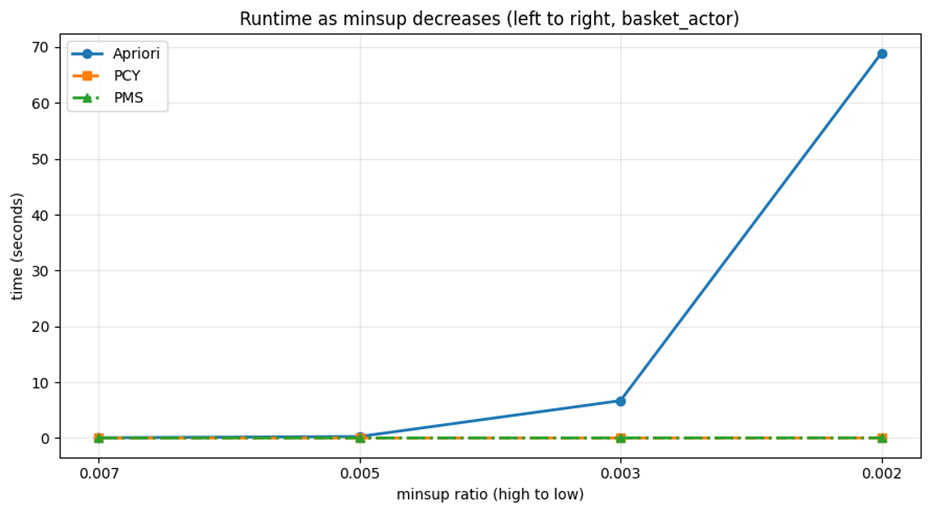
\includegraphics[width=0.65\linewidth]{figures/fig-6.png}
   
    \label{fig:6}
\end{figure}


\subsubsection{Algorithm behavior on enriched baskets}

On enriched baskets (actors plus a small number of movie attributes), the candidate space at low support grows much larger, making pruning more critical. Table~\ref{tab:14candidate_reduction_enriched} shows that at \(\mathrm{minsup} = 2\) all methods face \(7471\) candidate pairs, but PMS begins to deliver substantial savings once support increases: at \(\mathrm{minsup} = 5\) it cuts \(C_{2}\) from \(1230\) (Apriori) to \(547\),
and at \(\mathrm{minsup} = 10\) it still removes roughly \(42\%\) of Apriori's candidates. The combined candidate trends for Apriori, PCY, and PMS on enriched baskets are visualized in Figure~\ref{fig:7}, which highlights that multistage hashing is most beneficial in regimes where many pairs are close to the support threshold.

Runtime results in Table~\ref{tab:15runtime_speedup_enriched_final} and
Figure~\ref{fig:8} mirror these patterns. At \(\mathrm{minsup\_ratio} = 0.002\), both PCY and PMS are roughly 4 times faster than Apriori, reflecting the large candidate reductions, while at medium to high support the three algorithms converge to similar runtimes and PCY/PMS can even be slightly slower because the cost of hashing outweighs the smaller number of counted pairs. This behavior is consistent with the theoretical expectation that hashing is most advantageous when memory pressure from \(C_{2}\) is high.

\begin{table}[!htbp]
    \caption{Candidate Reduction on Enriched Baskets}
    \centering
    \normalsize
    \setlength{\tabcolsep}{4pt}
    \renewcommand{\arraystretch}{1.1}
    \begin{tabular}{rrrrrr}
        \toprule
        \textbf{minsup\_ratio} & \textbf{minsup} &
        \textbf{C2 (Apriori)} & \textbf{C2 (PCY)} &
        \textbf{C2 (PMS)} & \textbf{PMS Reduction (\%)} \\
        \midrule
        0.002 & 2  & 7471 & 7471 & 7340 & 1.75\%  \\
        0.005 & 5  & 1230 & 1226 & 547  & 55.53\% \\
        0.010 & 10 & 243  & 236  & 141  & 41.98\% \\
        0.030 & 30 & 115  & 109  & 109  & 5.22\%  \\
        0.050 & 50 & 115  & 106  & 100  & 13.04\% \\
        \bottomrule
    \end{tabular}%
    \label{tab:14candidate_reduction_enriched}
\end{table}

\begin{table}[!htbp]
    \caption{Runtime and Speedup of PCY and PMS Relative to Apriori (Enriched Baskets)}
    \centering
    \normalsize
    \setlength{\tabcolsep}{2.5pt}
    \renewcommand{\arraystretch}{1.08}
    \begin{tabularx}{\textwidth}{>{\centering\arraybackslash}p{0.11\textwidth} >{\centering\arraybackslash}p{0.08\textwidth} >{\centering\arraybackslash}X >{\centering\arraybackslash}X >{\centering\arraybackslash}X >{\centering\arraybackslash}X >{\centering\arraybackslash}X}
        \toprule
        \textbf{minsup\_ratio} & \textbf{minsup} &
        \textbf{time\_Apriori (s)} &
        \textbf{time\_PCY (s)} &
        \textbf{time\_PMS (s)} &
        \textbf{speedup\_PCY / Apriori} &
        \textbf{speedup\_PMS / Apriori} \\
        \midrule
        0.002 & 2  & 78.71 & 19.18  & 18.39  & 4.10 & 4.28 \\
        0.005 & 5  &  0.63 &  0.24  &  0.26  & 2.62 & 2.42 \\
        0.010 & 10 &  0.15 &  0.15  &  0.15  & 0.98 & 1.00 \\
        0.030 & 30 &  0.07 &  0.08  &  0.09  & 0.86 & 0.78 \\
        0.050 & 50 &  0.05 &  0.06  &  0.07  & 0.88 & 0.76 \\
        \bottomrule
    \end{tabularx}
    \label{tab:15runtime_speedup_enriched_final}
\end{table}

\begin{figure}[!htbp]
    \centering
    \caption{Enriched-basket comparison: candidate reduction and runtime behavior.}
    \label{fig:7-8}
    \begin{subfigure}[t]{0.49\textwidth}
        \centering
        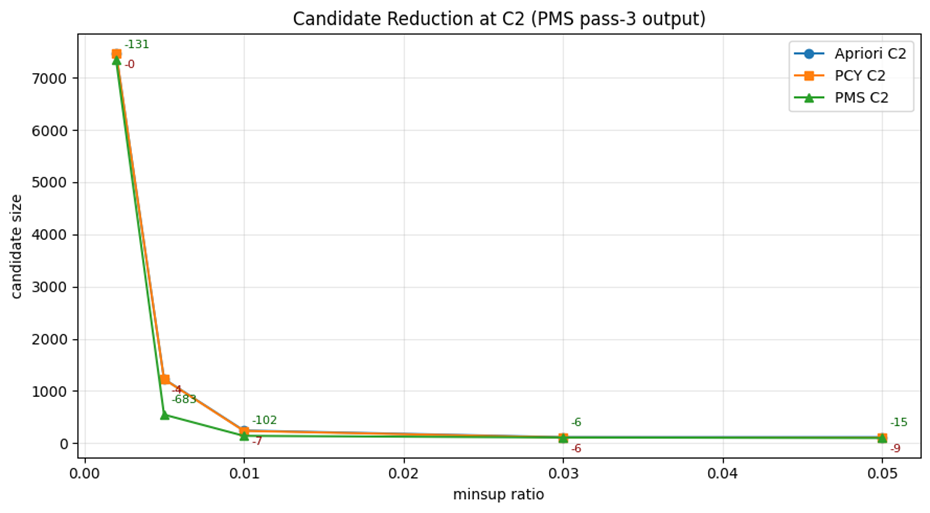
\includegraphics[width=\linewidth]{figures/fig-9a.png}
        \caption{Candidate generation reduction of PMS/PCY relative to Apriori (Enriched Baskets).}
        \label{fig:7}
    \end{subfigure}\hfill
    \begin{subfigure}[t]{0.49\textwidth}
        \centering
        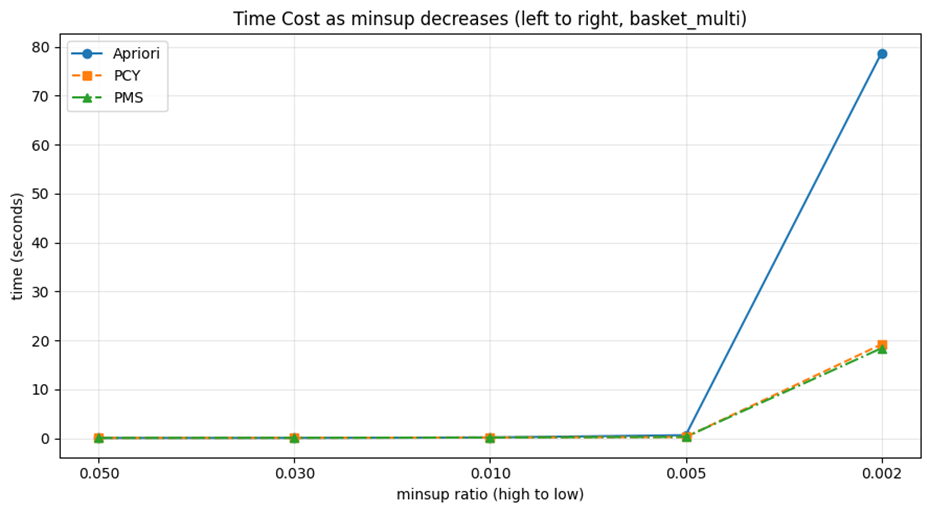
\includegraphics[width=\linewidth]{figures/fig-9b.png}
        \caption{Runtime comparison between Apriori and PCY (Enriched Baskets).}
        \label{fig:8}
    \end{subfigure}
\end{figure}

\subsubsection{Final configuration}

\FloatBarrier
Taken together, these experiments support the following configuration choices. On actor-only baskets, all three algorithms are correct but differ in efficiency: PCY reduces the candidate space significantly and delivers the best runtime across support thresholds, while PMS yields the most aggressive \(C_{2}\) pruning at the price of an extra pass and only modest additional speedup on this dataset size. On enriched baskets, multistage hashing (PMS) becomes more attractive at low support because the candidate space is much larger; however, once support is moderate or high, the runtime advantage over PCY and even Apriori largely disappears.

Given these observations and the underlying algorithmic trade-offs (monotonicity-based pruning in Apriori versus hash-based pruning in PCY/PMS),
I adopt PCY on actor-only baskets as the default configuration for the final rule-mining stage. Concretely, I fix \(\mathrm{minsup\_ratio} = 0.005\) (with absolute \(\mathrm{minsup}\) derived from the number of movies \(m\)) and \(\mathrm{minconf} = 0.50\), which provides enough support for interpretable rules while keeping frequent-pair mining computationally tractable (as in Table \ref{tab:16config_enriched}).
\begin{table}[!htbp]
    \caption{Final Configurations for Association Rule Mining}
    \centering
    \normalsize
    \setlength{\tabcolsep}{4pt}
    \renewcommand{\arraystretch}{1.1}

    \begin{subtable}[t]{0.48\textwidth}
        \centering
        \caption{ Actor-only baskets}
        \begin{tabularx}{\linewidth}{>{\raggedright\arraybackslash}p{0.38\linewidth}X}
            \toprule
            \textbf{Setting} & \textbf{Choice} \\
            \midrule
            Baskets & Actor-only (movies \(\rightarrow\) sets of actors) \\
            Algorithm & PCY \\
            minsup\_ratio & 0.005 \\
            minsup (absolute) & \(\lfloor 0.005 \cdot m \rfloor\) \\
            minconf & 0.50 \\
            \bottomrule
        \end{tabularx}
        \label{tab:config_actor_only}
    \end{subtable}
    \hfill
    \begin{subtable}[t]{0.48\textwidth}
        \centering
        \caption{Enriched baskets}
        \begin{tabularx}{\linewidth}{>{\raggedright\arraybackslash}p{0.38\linewidth}X}
            \toprule
            \textbf{Setting} & \textbf{Choice} \\
            \midrule
            Baskets & Enriched (actors + selected movie attributes) \\
            Algorithms & Apriori, PCY, PMS \\
            minsup\_ratio & \(\{0.002, 0.005, 0.01, 0.03, 0.05\}\) \\
            minsup (absolute) & \(\lfloor \text{minsup\_ratio}\cdot m \rfloor\) \\
            minconf & 0.50 (for rule-mining runs) \\
            \bottomrule
        \end{tabularx}
        \label{tab:16config_enriched}
    \end{subtable}
\end{table}

\section{Association Rules Mining}

\subsection{Rule Mining Configuration}
The final rule-mining configuration used for reporting is fixed to Table \ref{tab:17rule_mining_config}:

\begin{table}[!htbp]
    \caption{Rule-Mining Configuration}
    \centering
    \begin{tabular}{lrrrr}
        \toprule
        \textbf{Baskets} & \textbf{Algorithm} & \textbf{minsup ratio}&\textbf{minsup}  
 &minconf\\
        \midrule
        Actor-only   & PCY & 0.005&5   
 &0.5\\
        Enriched     & PMS & 0.05&50   &0.5\\
        \bottomrule
    \end{tabular}
    \label{tab:17rule_mining_config}
\end{table}
\subsection{Rule Metrics}

Rules are then generated from frequent itemsets mined under this setup, following the classical association-rule framework \parencite{yanCONFIDENCEMETRICSASSOCIATION2009}, the notebook computes: 

\begin{itemize}
    \item \textbf{Support} (joint frequency):
    \[
    \mathrm{supp}(X \Rightarrow Y)
    = \mathrm{supp}(X \cup Y)
    = \frac{\bigl|\{\,i : X \cup Y \subseteq T_{i}\,\}\bigr|}{m}.
    \]

    \item \textbf{Confidence} (directional reliability, \(P(Y \mid X)\)):
    \[
    \mathrm{conf}(X \Rightarrow Y)
    = \frac{\mathrm{supp}(X \cup Y)}{\mathrm{supp}(X)}.
    \]

    \item \textbf{Lift} (association strength vs.\ independence):
    \[
    \mathrm{lift}(X \Rightarrow Y)
    = \frac{\mathrm{conf}(X \Rightarrow Y)}{\mathrm{supp}(Y)}
    = \frac{\mathrm{supp}(X \cup Y)}
           {\mathrm{supp}(X)\,\mathrm{supp}(Y)}.
    \]

    \item \textbf{Interest (leverage)} (absolute deviation from independence) \parencite{InterestMeasureCalculateAdditional}:
    \[
    \mathrm{interest}(X \Rightarrow Y)
    = \mathrm{supp}(X \cup Y)
    - \mathrm{supp}(X)\,\mathrm{supp}(Y).
    \]

    \item \textbf{Kulczynski (KULC)} (average of directional confidences):
    \[
    \mathrm{Kulc}(X, Y)
    = \tfrac{1}{2}\bigl(P(Y \mid X) + P(X \mid Y)\bigr),
    \]
where values near 1 or 0 indicate strong positive or negative association and values near 0.5 indicate weak or uninteresting rules.

    \item \textbf{Fisher's exact test} \parencite{StatisticalNotesClinical}
 To reduce the chance of spurious rules, I additionally apply a one-sided
Fisher's exact test (alternative = ``greater'') on the \(2 \times 2\)
contingency table
\[
\begin{bmatrix}
a & b \\
c & d
\end{bmatrix}
=
\begin{bmatrix}
|X \cap Y|      & |X \cap \lnot Y| \\
|\lnot X \cap Y| & |\lnot X \cap \lnot Y|
\end{bmatrix},
\]
and keep only rules with \(p < 0.05\), which indicates that \(X\) and \(Y\)
co-occur significantly more often than expected under independence.

\end{itemize}

All above-mentioned metrics follow standard rule-interestingness practice in data mining and are summarized in Table~\ref{tab:8} and from previous work of \citeauthor{TanPNSteinbach} in Introduction to Data Mining, 2008.

\subsection{ Filtering and ranking policy}

Based on previous work in "Mining Top K Non-redundant Association Rules" of \cite{fournier-vigerMiningTopKNonredundant2012}, I adopt the ``interest for filtering, lift for ranking'' strategy that first enforces hard constraints and then orders the remaining rules:
\begin{table}[!htbp]
    \caption{Filtering and ranking policy for association rules}
    \centering
    \normalsize
    \setlength{\tabcolsep}{4pt}
    \renewcommand{\arraystretch}{1.15}
    \begin{tabularx}{\textwidth}{
        >{\centering\arraybackslash}p{0.06\textwidth}
        >{\raggedright\arraybackslash}p{0.20\textwidth}
        >{\raggedright\arraybackslash}X
    }
        \toprule
        \textbf{No.} & \textbf{Step} & \textbf{Description} \\
        \midrule
        1 & Filter by support &
        Discard rules with \(\mathrm{supp}(X \cup Y) < s_{\min}\) to ensure each
        rule is based on a sufficient number of baskets. \\

        2 & Filter by confidence &
        Discard rules with \(\mathrm{conf}(X \Rightarrow Y) < c_{\min}\) so that
        the consequent occurs often enough when the antecedent is present. \\

        3 & Filter by interest &
        Keep only rules with
        \(\lvert \mathrm{interest}(X \Rightarrow Y) \rvert \ge \iota_{\min}\),
        removing rules that are explained purely by the marginal popularity of
        \(X\) or \(Y\). \\

        4 & Filter by Fisher significance &
        Apply Fisher's exact test and discard rules with two-sided
        \(p \ge \alpha\) (here \(\alpha = 0.05\)), retaining only statistically
        significant departures from independence. \\

        5 & Remove redundant rules &
        Prune rules for which there exists a more specific rule
        \(X' \Rightarrow Y'\) with \(X \subset X'\), \(Y \subseteq Y'\), and
        identical support and confidence; such rules do not add new information. \\

        6 & Apply maximal antecedent filter &
        For a fixed consequent \(Y\), keep only rules whose antecedent \(X\) is
        inclusion-maximal among non-redundant rules with comparable
        support/confidence, so that each reported rule uses the largest
        informative context for predicting \(Y\). \\

        7 & Ranking (after filtering) &
        On the surviving set, rank rules primarily by lift, breaking ties by
        higher confidence and then by higher interest to surface rules that are
        strongly associated (high lift), reliable (high confidence), and
        substantially above chance co-occurrence (high interest). \\
        \bottomrule
    \end{tabularx}
    \label{tab:18filter_rank_policy}
\end{table}



\FloatBarrier
On the surviving set, I rank rules primarily by lift, breaking ties by higher
confidence and then by higher interest, which surfaces rules that are both
strongly associated (high lift), reliable (high confidence), and substantially
above chance co-occurrence (high interest). 

In practice, I read rules by first checking support (sufficient number of examples), then confidence, then interest and KULC to rule out popularity effects, and finally the Fisher \(p\)-value, before applying redundancy and maximality filters and ranking the remaining rules for reporting.  In the experiments, I retain only rules that satisfy \(\mathrm{supp\_count}(X \cup Y) \ge s_{\min}\) and
\(\mathrm{conf}(X \Rightarrow Y) \ge c_{\min}\) and that have a one-sided Fisher \(p\)-value below \(0.05\), so that the reported rules are frequent enough, sufficiently strong, and statistically
significant under an independence null model.

\subsection{Rules Analysis}

\subsubsection{Actor-only Baskets}

Before analyzing individual rules, I fix a single PCY configuration on actor-only baskets and summarize it in Table~\ref{tab:19config_summary}. With \(\text{minsup\_ratio} = 0.005\) (i.e., \(\text{minsup} = 5\) movies), 79 actors remain frequent in \(L_1\); PCY then generates 51 candidate pairs \(C_2\), of which only 3 pairs are frequent in \(L_2\), all found in 0.026 seconds. Using hash buckets ensures that most non-promising pairs are pruned at the hashing stage while preserving all truly frequent actor--actor pairs for subsequent rule mining.


\begin{table}[!htbp]
    \caption{Configuration summary of association-rule mining run (Actor-only Baskets)}
    \centering
    \begin{tabular}{l r}
        \toprule
        \textbf{Quantity} & \textbf{Value} \\
        \midrule
        minsup\_ratio   & 0.005 \\
        minsup          & 5 \\
        L1\_size        & 79 \\
        C2\_size        & 51 \\
        L2\_size        & 3 \\
        time\_sec       & 0.02583 \\
        num\_buckets    & 2048 \\
        freq\_buckets   & 365 \\
        \bottomrule
    \end{tabular}
    \label{tab:19config_summary}
\end{table}

For actor‑only baskets, the strongest rules are pure actor–actor co‑occurrences and recover well‑known franchise structure. The top five rules (Table \ref{tab:20actor_only_rules}) all involve the Harry Potter trio (Daniel Radcliffe, Rupert Grint, Emma Watson) with support between 0.005 and 0.006, confidence between 0.714 and 1.000, and extremely high lift (approximately 120–167), indicating that whenever one of these actors appears, the others are present far more often than chance would predict. The frequent triple \textit{\{Radcliffe, Watson, Grint\}} appears in 5 of 1000 movies, exactly matching the main Harry Potter entries in the Top‑1000 subset, and illustrates that the actor‑only configuration captures franchise‑level patterns with very high directional reliability. 
\begin{table}[!htbp]
    \caption{Top 5 actor--actor rules in actor-only baskets}
    \centering
    \begin{tabular}{l l r r r r r}
        \toprule
        \textbf{lhs} & \textbf{rhs} &
        \textbf{support\_count} & \textbf{support} &
        \textbf{confidence} & \textbf{lift} &
        \textbf{interest} \\
        \midrule
        daniel radcliffe & rupert grint &
        6 & 0.006 & 1.000000 & 166.666667 & 0.005964 \\
        rupert grint & daniel radcliffe &
        6 & 0.006 & 1.000000 & 166.666667 & 0.005964 \\
        daniel radcliffe & emma watson &
        5 & 0.005 & 0.833333 & 119.047619 & 0.004958 \\
        rupert grint & emma watson &
        5 & 0.005 & 0.833333 & 119.047619 & 0.004958 \\
        emma watson & daniel radcliffe &
        5 & 0.005 & 0.714286 & 119.047619 & 0.004958 \\
    \end{tabular}
    \label{tab:20actor_only_rules}
\end{table}

\begin{table}[!htbp]

    \caption{Frequent actor triples (L3) in actor-only baskets}
    \centering
    \begin{tabular}{l r r}
        \toprule
        \textbf{triple} & \textbf{support\_count} & \textbf{support} \\
        \midrule
        (daniel radcliffe, emma watson, rupert grint) & 5 & 0.005 \\
        \bottomrule
    \end{tabular}
    \label{tab:21frequent_triples}
    
\end{table}

\subsubsection{Enriched Baskets}
For enriched baskets, I move from actor-only baskets to baskets that combine actors with discretized success features (gross, votes, rating, runtime, metascore tiers) and run PMS with two support settings (Config A and Config B in Table~\ref{tab:22config_comparison}). Config A uses \(\text{minsup\_ratio} = 0.01\) (\(\text{minsup} = 10\) movies) to expose more candidate patterns, while Config B uses a stricter \(\text{minsup\_ratio} = 0.05\) (\(\text{minsup} = 50\) movies) to focus on highly supported rules; both share \(\text{minconf} = 0.5\), \(k_{\max} = 9\), 4,096 hash buckets, and a \(p\)-value threshold of 0.05.

\begin{table}[!htbp]
    \caption{Association-rule mining configurations}
    \centering
    \begin{tabular}{l r r}
        \toprule
        \textbf{Parameter} & \textbf{Config A} & \textbf{Config B} \\
        \midrule
        n\_baskets   & 1000 & 1000 \\
        minsup\_ratio & 0.01 & 0.05 \\
        minsup       & 10   & 50   \\
        minconf      & 0.5  & 0.5  \\
        max\_k       & 9    & 9    \\
        num\_buckets & 4096 & 4096 \\
        p\_threshold & 0.05 & 0.05 \\
        \bottomrule
    \end{tabular}
    \label{tab:22config_comparison}
\end{table}


Table~\ref{tab:23rule_pipeline_counts_combined} shows how the filtering pipeline compresses the rule set at these two supports. At \(\text{minsup\_ratio} = 0.01\), 475 rules pass the basic configuration; Fisher’s test removes only a small fraction (retaining 97.7\%), but redundancy and maximality pruning are much stronger, leaving 160 final rules (about 34\% of the original). At \(\text{minsup\_ratio} = 0.05\) the search starts from only 46 rules, all of which are significant by Fisher; the structural filters again remove many near-duplicates, leaving 31 final rules (about 67\% retention), with most surviving rules being multi-item antecedents targeting a small number of consequents.
\begin{table}[!htbp]
    \caption{ Rule counts at successive filtering stages}
    \centering
    \begin{tabular}{l r r r r}
        \toprule
        & \multicolumn{2}{c}{\textbf{minsup\_ratio = 0.01}} &
          \multicolumn{2}{c}{\textbf{minsup\_ratio = 0.05}} \\
        \textbf{Stage}&
        \textbf{Rules} & \textbf{Retention (\%)} &
        \textbf{Rules} & \textbf{Retention (\%)} \\
        \midrule
        raw\_after\_configuration        & 475 & 100.00 & 46 & 100.00 \\
        after\_fisher\_test\_significance & 464 & 97.68  & 46 & 100.00 \\
        after\_non\_redundant            & 300 & 63.16  & 37 & 80.43 \\
        after\_maximal (final rules)     & 160 & 33.68  & 31 & 67.39 \\
        final\_1\_to\_1                  & 7   & 1.47   & 1  & 2.17  \\
        final\_n\_to\_1                  & 153 & 32.21 & 30 & 65.22 \\
        \bottomrule
    \end{tabular}
    \label{tab:23rule_pipeline_counts_combined}
\end{table}


Within this setup, the clearest single-actor signal is \(\texttt{actor:tom hanks} \Rightarrow \texttt{gross\_tier:high}\) (Table~\ref{tab:24tom_hanks_gross_high_rule}). The rule has support \(14/1000\), confidence 1.0, lift 3.61, interest 0.0101, a two-sided Fisher \(p\)-value around \(1.2 \times 10^{-8}\), and Kulczynski \(\approx 0.53\), indicating a strong, statistically significant association between Tom Hanks and high-gross movies beyond what the marginal frequencies would suggest. The supporting titles \emph{Forrest Gump}, \emph{Saving Private Ryan}, \emph{The Green Mile}, \emph{Toy Story}, \emph{Toy Story 3}are all well-known high-revenue films, which makes this rule a sanity check that the enriched configuration can recover intuitive star-success relationships.

\begin{table}[!htbp]
    \caption{Top One-Item 1$\rightarrow$1 rule for \texttt{gross\_tier:high} and supporting movies}
    \centering

    % Top rule
    \begin{subtable}{\linewidth}
        \centering
        \setlength{\tabcolsep}{2.5pt}
        \renewcommand{\arraystretch}{1.08}
        \begin{adjustbox}{max width=\linewidth}
        \begin{tabular}{p{0.20\linewidth} p{0.16\linewidth} r r r r r r r}
            \toprule
            \textbf{Antecedent} & \textbf{Consequent} &
            \textbf{supp\_cnt} & \textbf{supp} &
            \textbf{conf} & \textbf{lift} &
            \textbf{interest} & \textbf{p-value} & \textbf{Kulc} \\
            \midrule
            actor:tom hanks & gross\_tier:high &
            14 & 0.014 & 1.0 & 3.610108 &
            0.010122 & 1.23$\times 10^{-8}$ & 0.525271 \\
            \bottomrule
        \end{tabular}
        \end{adjustbox}
    \end{subtable}

    \vspace{0.5em}

    % Top 5 supporting movies
    \begin{subtable}{\linewidth}
        \centering
        \begin{tabular}{l r}
            \toprule
            \textbf{Title} & \textbf{Year} \\
            \midrule
            Forrest Gump        & 1994 \\
            Saving Private Ryan & 1998 \\
            The Green Mile      & 1999 \\
            Toy Story           & 1995 \\
            Toy Story 3         & 2010 \\
            \bottomrule
        \end{tabular}
    \end{subtable}

    \label{tab:24tom_hanks_gross_high_rule}
\end{table}


Multi-item rules for \(\text{gross\_tier:high}\) further refine this picture by combining actor and feature information (Table~\ref{tab:25top_ng1_gross_high_with_subtables}). For instance, \(\{\text{meta\_score\_tier:low}, \text{runtime\_tier:high}\} \Rightarrow \text{gross\_tier:high}\) has support 0.016, confidence 1.0, lift 3.61, and a very small \(p\)-value, suggesting that long, modestly reviewed films in this sample tend disproportionately to be high-gross blockbusters (e.g., \emph{The Hobbit: An Unexpected Journey}, \emph{Rogue One}, \emph{Captain America: The Winter Soldier}). 

Similarly, rules like:

\[
\begin{aligned}
\{\texttt{actor:matt damon},\ \texttt{votes\_tier:high}\} &\Rightarrow \texttt{gross\_tier:high},\\
\{\texttt{actor:leonardo dicaprio},\ \texttt{votes\_tier:high}\} &\Rightarrow \texttt{gross\_tier:high}.
\end{aligned}
\]

show that when these actors appear in highly voted films, those films are almost always in the high-gross tier (confidence 1.0, lift 3.61, highly significant \(p\)-values), reflecting a combination of star power and large audience reach.

\begin{table}[!htbp]
    \caption{Top N$\rightarrow$1 rules for \texttt{gross\_tier:high} and example high-grossing movies}
    \centering
    \normalsize
    \setlength{\tabcolsep}{3pt}
    \renewcommand{\arraystretch}{1.1}

    % Top 5 N->1 rules
    \begin{subtable}{\linewidth}
        \centering
        \caption{Top 5 N$\rightarrow$1 rules for \texttt{gross\_tier:high}}
        \begin{adjustbox}{max width=\linewidth}
        \begin{tabular}{p{0.33\linewidth} p{0.13\linewidth} r r r r r r r}
            \toprule
            \textbf{Antecedent} & \textbf{Consequent} &
            \textbf{supp\_cnt} & \textbf{supp} &
            \textbf{conf} & \textbf{lift} &
            \textbf{interest} & \textbf{p-value} & \textbf{Kulc} \\
            \midrule
            \{meta\_score\_tier:low, runtime\_tier:high\} &
            gross\_tier:high &
            16 & 0.016 & 1.000000 & 3.610108 &
            0.011568 & \(8.72\times 10^{-10}\) & 0.528881 \\
            \{actor:matt damon, votes\_tier:high\} &
            gross\_tier:high &
            10 & 0.010 & 1.000000 & 3.610108 &
            0.007230 & \(2.36\times 10^{-6}\) & 0.518051 \\
            \{actor:leonardo dicaprio, votes\_tier:high\} &
            gross\_tier:high &
            10 & 0.010 & 1.000000 & 3.610108 &
            0.007230 & \(2.36\times 10^{-6}\) & 0.518051 \\
            \{actor:leonardo dicaprio, runtime\_tier:high\} &
            gross\_tier:high &
            10 & 0.010 & 1.000000 & 3.610108 &
            0.007230 & \(2.36\times 10^{-6}\) & 0.518051 \\
            \{runtime\_tier:high, rating\_tier:mid, votes\_tier:high\} &
            gross\_tier:high &
            13 & 0.013 & 0.928571 & 3.352243 &
            0.009122 & \(4.83\times 10^{-7}\) & 0.487751 \\
            \bottomrule
        \end{tabular}
        \end{adjustbox}
    \end{subtable}

    \vspace{0.3em}

    % Top 5 example movies
    \begin{subtable}{\linewidth}
        \centering
        \caption{Example high-grossing movies matching the top rule}
        \begin{adjustbox}{max width=\linewidth}
        \begin{tabular}{p{0.82\linewidth} r}
            \toprule
            \textbf{Title} & \textbf{Year} \\
            \midrule
            \multicolumn{2}{p{0.97\linewidth}}{\textit{Movies matching top N$\rightarrow$1 rule:
            \{meta\_score\_tier:low, rating\_tier:low, runtime\_tier:high, votes\_tier:high\}
            \(\rightarrow\) \{gross\_tier:high\}}} \\
            \addlinespace[0.3em]
            The Hobbit: An Unexpected Journey & 2012 \\
            Rogue One & 2016 \\
            Harry Potter and the Deathly Hallows: Part 1 & 2010 \\
            Captain America: The Winter Soldier & 2014 \\
            Star Trek Into Darkness & 2013 \\
            \bottomrule
        \end{tabular}
        \end{adjustbox}
    \end{subtable}

    \label{tab:25top_ng1_gross_high_with_subtables}
\end{table}


\FloatBarrier
Taken together, the rule-mining configuration and filtering pipeline yield a small, interpretable set of statistically supported associations that align with domain intuition. 

\begin{itemize}
    \item     \textit{Actor-only baskets}:  mined with PCY at low support, mainly recover very high-lift franchise co-occurrences such as the Harry Potter trio, showing that hashing-based pair mining can compress candidate sets without losing meaningful collaborations.
    \item     \textit{Enriched baskets:} extend this picture by combining actors with discretized success tiers, where the “interest for filtering, lift for ranking” strategy and Fisher’s test remove popularity-driven and redundant rules and highlight patterns like Tom Hanks’ consistent presence in high-gross titles and multi-feature signatures of blockbuster performance.

\end{itemize}
Overall, the experiments illustrate how classical interestingness measures, significance testing, and maximal non-redundant pruning can turn a large raw rule pool into a focused set of movie-success rules that are both statistically sound and easy to interpret.


\section{Discussion and Conclusion}

\subsection{Key Empirical Takeaways}

From the algorithm experiments, the main empirical finding is that PCY-style hashing behaves as predicted in the literature: it preserves the frequent pairs found by Apriori while reducing the number of counted candidate pairs (\(C_2\)), especially on enriched, higher-dimensional baskets. On actor-only baskets, this pruning is already visible in runtime at low support (for example, minsup \(=2\): Apriori \(\approx 65.15\)s vs PCY \(\approx 0.013\)s and PMS \(\approx 0.014\)s), while gaps narrow as minsup increases. On enriched baskets (actors plus tier features), PCY and PCY-Multistage again produce smaller candidate sets and lower pair-mining runtimes under the same 2048-bucket budget.

On the rule-mining side, the final configured run (actor-only, PCY, minsup ratio \(0.005\), minconf \(0.50\)) yields a compact and interpretable rule set. The surviving rules are mainly high-lift actor--actor links that match known collaborations, while stricter significance/redundancy/maximal filtering removes most weak or duplicated patterns. This supports the view that even this top-1000 IMDB sample contains non-trivial association structure.

\subsection{Limitations of Data and Methods}

The first limitation is dataset size. The IMDB Top-1000 subset has only 1000 baskets with four main actors per movie, so both the pattern space and the range of meaningful minsup values are limited. Although low-minsup runs can still be expensive for Apriori in this implementation, the dataset does not fully stress the true ``massive data'' regime discussed in MMDS (e.g., distributed I/O and cluster-scale memory pressure).

A second limitation is the inherent combinatorial hardness of frequent-itemset mining. The number of frequent itemsets can grow exponentially with the number of items, so no single method can avoid hard cases in general \cite{aroraComputationalComplexityModern2009}. In practice, scalability depends on problem-specific choices: sensible minsup/minconf thresholds, strong pruning (downward closure, hashing, leverage-based filtering), and, for very large datasets, acceptance of heuristic or approximate methods when exact enumeration becomes too costly.

\subsection{Possible Extensions and Future Work}

A direct extension is larger data coverage (for example, a larger IMDB/TMDB corpus) to better evaluate memory usage, candidate growth, and runtime across broader minsup and bucket settings. With millions of baskets and a richer actor/feature vocabulary, the comparison between Apriori, PCY, and PCY-Multistage would be more representative of truly large-scale mining.

On the algorithmic side, FP-Growth is a strong follow-up baseline. Instead of explicit candidate generation, FP-Growth compresses transactions into an FP-tree and mines patterns through conditional pattern bases and depth-first recursion. Comparing FP-Growth against Apriori/PCY/PMS on the same movie baskets would clarify when tree-based compression outperforms hash-based pruning.

Another extension is graph-based analysis of mined associations: treat actors and feature tiers as nodes, and high-lift/high-interest relations as edges. Community detection, centrality, and motif analysis could reveal collaboration clusters and success-related structures that are less visible in rule tables alone.

\subsection{Reproducibility}

All experiments in this project are implemented in a single notebook and driven by a small set of global configuration knobs printed at the top (e.g., \verb|SEED = 42|, \verb|DEFAULT_NUM_BUCKETS = 2048|, and minsup grids for each dataset). The full pipeline from data loading and cleaning, through basket construction and algorithm comparison, to rule mining and post-processing runs end-to-end on the same cleaned IMDB dataset table, with intermediate tables and plots generated directly from code rather than edited by hand. This design, combined with fixed random seeds and explicit parameter logs, makes it straightforward to rerun all experiments on another machine, or to re-execute the notebook with different minsup/bucket settings or alternative datasets in future work.



\section*{Acknowledgement}

\textit{I/We declare that this material, which I/We now submit for assessment, is entirely my/our own work and has not been taken from the work of others, save and to the extent that such work has been cited and acknowledged within the text of my/our work, and including any code produced using generative AI systems. I/We understand that plagiarism, collusion, and copying are grave and serious offences in the university and accept the penalties that would be imposed should I engage in plagiarism, collusion or copying. This assignment, or any part of it, has not been previously submitted by me/us or any other person for assessment on this or any other course of study.}
\clearpage
\nocite{*}
\printbibliography



\end{document}

/














